\cotefile{45}
\scanpage{33}
\margin{32}
- \mspage{22} - \hfill n$^{\mathrm{o}}$ 246

la réunion de $]\Delta_1,\Delta_2[$, de $\Delta_1$ et de $\Delta_2$.

\uline{Lorsque} $k$ \uline{satisfait à l'hypothèse du chapeau du n$^{\mathrm{o}}$} 6, on peut, au moyen d'une forme quadratique auxiliaire, établir une correspondance biunivoque \uline{croissante} entre le corps $k$ et l'ensemble ordonné défini par la prop. 6. [N.B. Pour le cas où $k$ ne satisfait pas à l'hypothèse en question, l'adjudant de service fabriquera un contre-exemple et le mettra en exercice]. Pour cela, on introduit dans le plan $E$ n'importe quelle forme quadratique $\phi$ pour laquelle $-\delta$ est un carré, ce qui nous permet d'appliquer tous les résultats des n$^{\mathrm{os}}$ précédents. Pour toute demi-droite $\Delta$ autre que $\Delta_0$, on posera
\[
t(\Delta)=\operatorname{tg}\frac12(-\Delta_0,\Delta).
\]
Comme on a $\Delta\ne\Delta_0$, $(-\Delta_0,\Delta)$ n'est pas l'angle plat, donc $\frac12(-\Delta_0,\Delta)$ n'est pas un angle droit et par suite $t(\Delta)\ne\infty$. Il est immédiat que $\Delta\longrightarrow t(\Delta)$ est une bijection de l'ensemble des demi-droites $\ne\Delta_0$ sur $k$. On va montrer que cette bijection est croissante. Soient en effet $\Delta_1,\Delta_2$ deux demi-droites distinctes de $\Delta_0$ ; soit $t_i=t(\Delta_i)$ $(i=1,2)$
Soit $a$ un point, autre que $0$, sur $-\Delta_0$ ; pour la base $(a,Ja)$ de $E$, les demi-droites $\Delta_0,\Delta_1,\Delta_2$ contiendront respectivement (en vertu de la formule (12)) les points :
\[
\begin{aligned}
x_0&=(-1,0),\\
x_i&=(1-t_i^2,2t_i)\quad(i=1,2),
\end{aligned}
\]
Pour que la suite $\Delta_0,\Delta_1,\Delta_2$ soit directe, il faut et il suffit que deux au moins des quantités
\[
-2t_1,\quad(1-t_1^2)2t_2-(1-t_2^2)2t_1,\quad2t_2
\]
soient $>0$. Or la seconde s'écrit $2(t_2-t_1)(1+t_1t_2)$.
\scanpage{34}
Soit $G$ un \inserted{\unsure{schéma en}} groupe affine sur $A$, $A$-\unsure{simple}
\[
\begin{array}{ll}
\operatorname{Aff}_A(G)&\text{son algèbre affine}\\[1ex]
U_A(G)&\text{son hyperalgèbre}
\end{array}
\]

Donc
\[
\left\{\begin{array}{l}
\operatorname{Aff}_A(G)\text{ est une }A\text{-algèbre commutative augmentée,}\\
\qquad\text{munie d'un hom diagonal multiplicatif,}\\
\qquad\text{associatif, compatible avec les augmentations}\\[1ex]
U_A(G)\text{ est une }A\text{-algèbre en général non comm.,}\\
\qquad\text{munie d'un hom diagonal multiplicatif,}\\
\qquad\text{associatif, comm. compatible avec les}\\
\qquad\text{augmentations}
\end{array}\right.
\]

Il y a un produit scalaire
\[
\langle f,X\rangle=\langle\deleted{\unsure{f}}\inserted{X},\deleted{\unsure{X}}\inserted{f}\rangle
\]
entre $\operatorname{Aff}_A(G)$ et $U_A(G)$, ce dernier s'identifiant aux formes $A$-linéaires sur $\operatorname{Aff}_A(G)$ qui s'annulent sur une puissance de l'idéal d'augmentation.

$U_A(G)$ opère à g. et à droite sur $\operatorname{Aff}_A(G)$ [qui est un bimodule sur $U_A(G)$]
\[
\left\{\begin{aligned}
\langle Y,X*f\rangle&=\langle Y*X,f\rangle=\langle f,Y*X\rangle=\langle f*Y,X\rangle\\
\langle\varepsilon,X*f\rangle&=\langle\varepsilon,f*X\rangle=\langle X,f\rangle
\end{aligned}\right.
\]
\margin{33}
\scanpage{35}
$\operatorname{Aff}_A(G)$ opère \deleted{à gauche et à droite} sur $U_A(G)$ ; les formules sont \deleted{\unsure{de la forme}} analogues
\[
\langle g,f\mathbin{\lrcorner}X\rangle=\langle gf,X\rangle
\qquad\text{en particulier }\langle f,X\rangle=\varepsilon(f\mathbin{\lrcorner}X)
\]

Supposons maintenant que $A\subset B$, alors
\[
\operatorname{Aff}_B(G)=\operatorname{Aff}_A(G)\otimes_A B\supset\operatorname{Aff}_A(G)
\]
[on a une \uline{inclusion}, car $\operatorname{Aff}_A(G)$ plat sur $A$]
\[
U_B(G)=U_A(G)\otimes_A B\supset U_A(G)
\]
[raison analogue ; la première égalité est due au fait que $G$ est $A$-simple]

\uline{Proposition 1} Soit $X\in U_B(G)$. Conditions équivalentes
\[
\begin{array}{ll}
\text{(i)}&X\in U_A(G)\\
\text{(ii)}&X*\operatorname{Aff}_A(G)\subset\operatorname{Aff}_A(G)
\qquad\text{(ii bis)}\ \operatorname{Aff}_A(G)*X\subset\operatorname{Aff}_A(G)\\
\text{(iii)}&\langle X,\operatorname{Aff}_A(G)\rangle\subset A
\end{array}
\]
En effet,
\diagram{\begin{tikzcd}[ampersand replacement=\&,column sep=small,row sep=small]
\&\text{(ii bis)}\arrow[dr,Rightarrow]\&\\
\text{(i)}\arrow[ur,Rightarrow]\arrow[r,Rightarrow]\&\text{(ii)}\arrow[r,Rightarrow]\&\text{(iii)}
\end{tikzcd}}
triviaux.

(iii) implique que \deleted{$\unsure{X\in U_A}$} \deleted{la forme} \inserted{$X$ définit} une forme $A$-linéaire sur $\operatorname{Aff}_A(G)$ nulle sur une puissance de l'idéal d'augmentation, donc un élément $X_0$ de $U_A(G)$, qui \unsure{n'est} évidemment \unsure{autre que} $X$
\margin{34}
\scanpage{36}
\uline{Proposition 2} Soit $f\in\operatorname{Aff}_B(G)$. \inserted{Supposons $G$ $A$-connexe.} Conditions équivalentes
\[
\begin{array}{ll}
\text{(i)}&f\in\operatorname{Aff}_A(G)\\
\text{(ii)}&f\mathbin{\lrcorner}U_A(G)\subset U_A(G)\\
\text{(iii)}&\langle f,U_A(G)\rangle\subset A
\end{array}
\]
\margin{\unsure{)}}

Évidemment
\diagram{\begin{tikzcd}[ampersand replacement=\&,column sep=small]
\text{(i)}\arrow[r,Rightarrow]\&\text{(ii)}\arrow[r,Rightarrow]\&\text{(iii)}
\end{tikzcd}}
[et
\diagram{\begin{tikzcd}[ampersand replacement=\&,column sep=small]
\deleted{\unsure{\text{(ii)}}}\inserted{\text{(iii)}}\arrow[r,Rightarrow]\&\text{(ii)}
\end{tikzcd}}
car \deleted{\unsure{soit}} $X\in U_A(G)$, pour prouver $f\mathbin{\lrcorner}X\in U_A(G)$ il suffit \inserted{(prop. 1)} de vérifier que $\langle g,f\mathbin{\lrcorner}X\rangle\in A$ pour $g\in\operatorname{Aff}_A(G)$, or
\[
\langle g,f\mathbin{\lrcorner}X\rangle=\langle gf,X\rangle=\langle f,g\mathbin{\lrcorner}X\rangle
\in\langle f,U_A(G)\rangle\subset A
\]
] Prouvons $(\mathrm{iii})\Rightarrow\mathrm{i})$ en utilisant que $G$ est $A$-connexe.

Soit $C_{\deleted{\unsure{A|B}}}=\operatorname{Aff}_A(G)$, considérons le diagramme
\diagram{\begin{tikzcd}[ampersand replacement=\&]
C\arrow[r]\arrow[d]\&C_B\arrow[d]\\
\widehat C\simeq\operatorname{Hom}_A(U,A)\arrow[r]\&\widehat C_B=\operatorname{Hom}_B(U_B,B)
\end{tikzcd}}
où $\widehat{\phantom C}$ désigne le \inserted{\unsure{séparé}} complété pour l'idéal d'augmentation.
\margin{35}
\scanpage{37}
\begin{flushright}
Cohomologie de l'algèbre\\
de Lie et \unsure{coh,|coh.} des\\
groupes \unsure{..-|...}
\end{flushright}
\margin{36}
\scanpage{38}
Soit $G$ un schéma en groupes simple sur $S=\operatorname{Spec}A$, $A$ Artinien loc.
\[
\mathfrak g=L_S(G)
\]

(1) Si $H^0(\mathfrak g_0,\mathfrak g_0)=0$, $\Longleftrightarrow$ $G\to\underline{\operatorname{Aut}}_S(\mathfrak g)$ est un \unsure{m. infi.}
[donc si $G_0$ n'a pas de sous-groupe \deleted{discret} étale \deleted{\unsure{fini invariant}} non trivial, alors c'est une \unsure{immersion} fermée]

(2) \deleted{Si} \inserted{(1) et} \deleted{de plus} $H^1(\mathfrak g_0,\mathfrak g_0)=0$ $\Longleftrightarrow$ \deleted{\unsure{donc}} $G\to\underline{\operatorname{Aut}}_S(\mathfrak g)$ est étale,
[alors sous la condition dite plus haut, c'est une immers. ouverte, donc $G\simeq\underline{\operatorname{Aut}}_S^0(\mathfrak g)$ si $G$ à fibres connexes]

\margin{\deleted{(1) et (2)} \unsure{(2)} $\Rightarrow\underline{\operatorname{Aut}}_S(\mathfrak g)\simeq\underline{\operatorname{Aut}}_S(G)$ si $G$ connexe\ldots\ Utilisant \unsure{Tôhoku} cela suffirait à construire les \unsure{Tchevalley} \deleted{\unsure{sur}} sur $\mathbb Z$\ldots}

Supposons qu'on ne dispose pas de $G$, mais seulement de $\mathfrak g$, considérons $H=\underline{\operatorname{Aut}}_S(\mathfrak g)$.
\deleted{Alors} C'est un schéma en groupes sur $S$, et $\operatorname{Lie}_k(H_0)=\mathfrak h_0$ est isomorphe à \deleted{$\unsure{\mathfrak g_0/(\text{centre de }\mathfrak g_0)}$ \unsure{par}} \inserted{l'algèbre de Lie des} \deleted{\illegible{2}} dérivations de $\mathfrak g_0$, d'où $\mathfrak g_0\to\mathfrak h_0$, qui est un \unsure{isom} si (1) et (2) sont satisfaites.

S'il en est ainsi, on ne peut affirmer encore que $H$ est simple sur $S$, \unsure{avec les hyp 1 2 seules citées}, \deleted{\unsure{Mais donc}} on le peut si on suppose
\[
\text{(3)}\qquad H^2(\mathfrak g_0,\mathfrak g_0)=0.
\]
qui signifie sauf erreur qu'il n'y a pas de variations de structure \inserted{infinitésimales} \unsure{non triviales} de $\mathfrak g_0$, et \uline{implique} que \deleted{\unsure{$H$ est donc}} $\underline{\operatorname{Aut}}_S(\mathfrak g)$ est simple sur $S$.
\margin{37}
\scanpage{39}
\margin{38}
que toute fonction rationnelle definie en $x$ soit definie en $y$. \deleted{Alors $\underline O_y$ domine} La condition est de toutes façons necessaire, prouvons qu'elle est suffisante (utilisant la separation). Supposons $\underline O_x\quad\underline O_y$, donc (\deleted{\unsure{l}}lemme 1) il existe un ideal premier $\underline p$de $\underline O_x$ tel que $\underline O_y$ domine $\underline O_{x\,\underline p}$. Or il existe un $z\quad X$ tel que $x\quad\bar z$, $\underline O_z=\underline O_{x\,\underline p}$ (\unsure{reference}
donc $\underline O_z$ et $\underline O_y$ sont apparentes, donc $z=y$ cqfd.

On peut reenoncer ce corollaire ainsi: si $x\notin\bar y$, il existe une fonction rationnelle $f$ sur $X$ telle que $f$ soit definie en $x$ et non en $y$ i.e. telle que $D(f)$ contienne $x$ et ne rencontre pas $\bar y$. Si maintenant $X$ est un espace noetherien, toute partie fermee de $X$ est reunion finie de fermes irreductibles, i.e. de la forme $\bar y$, d'ou:

\uline{Corollaire} 3 Soit $X$ un schema integre noetherien (il suffit de dire: qui est un espace topologique noeth.), alors les $D(f)$ forment une base de la topologie de $X$.

On voit ainsi comment la topologie de $X$, identifie a un ensemble de sous-anneaux locaux de $R$, peut se recuperer en termes de cette derniere structure; de façon equivalente, on peut aussi remarquer que la topologie de $X$ est definie entermes de sastructure d'ordre, un \unsure{ferme} de $X$ etant forme des elements de $X$ majores par un au moins parmi les elements d'une partie finie de $X$ (la majoration etant definie \deleted{\unsure{sont}} ici en termes d'inclusions \deleted{de parties \unsure{de $R$}} d'anneaux locaux). D'autre part, le faisceau $\underline O_X$ lui aussi est recupere, puisque
\[
\mathrm I(U,\underline O_X)=\underline O_x\quad(x\quad U)
\]
Plus bas, nous donnerons quelques indications plus precis\deleted{\unsure{s}}es.

\uline{Proposition} 3 Soit $f:X\quad Y$ un morphisme dominant de schemas integres, \deleted{\unsure{de corps}} soit $L$ ($K$) le corps de $X$ ($Y$). Identifions $K$ a un sous-corps de $L$, et les anneaux locaux de $X$ ($Y$) a des sous-anneaux de $L$ ($K$). Alors pour tout $x\quad X$, $\underline O_{f(x)}$ est l'unique anneau local de $Y$ domine par $\underline O_x$.

Il est en effet domine, par definition d'un morphisme, et il est unique puisque deux anneaux locaux de $Y$ apparentes sont identiques.

\uline{Proposition} 4 Soit $f$ un morphisme \uline{separe} d'immersion locale (resp. d'isomorphisme local) de $X$ dans $Y$, avec \deleted{$Y$} $X$ \uline{irreductible}. Alors $f$ est une immersion (resp. une immersion ouverte).

Il suffit de montrer que $f$ est un homeomorphisme dans (ce qui impliquera facilement, compte tenu de l'hypothese, que $f(X)$ est localement ferme dans $Y$). On peut evidemment supposer $X$ et $Y$ \uline{reduits}, et on voit qu'on peut remplacer $Y$ par l'adherence de $f(X)$, donc on peut supposer $f$ dominant. Alors \deleted{$Y$ sera aussi} $Y$ sera aussi irreductible, donc $X$ et $Y$ sont integres. Avec les notations de prop.3, on aura pour tout $x\quad X$
\scanpage{40}
De plus, (1) (2) (3) [\unsure{impliquant|indiquant} l'existence d'un $G$ \unsure{simple} sur $S$ donnant $\mathfrak g$] prouvent aussi [pour $G$ connexe] que $G$ n'a pas de variations infinitésimales non triviales.

Question du relèvement de la structure $G$ \inserted{(connexe)}, équivaut à la question du relèvement de la structure $\mathfrak g$. On trouve une obstruction dans $H^3(\mathfrak g,\mathfrak g)$. Donc

\deleted{$H^3$}

(3) Si $H^3(\mathfrak g,\mathfrak g)=0$, alors on peut relever de façon \unsure{essentiellement} unique $\mathfrak g$, ou $G$ de façon équivalente.

\uline{Question} Définir
\[
H^{\unsure{*}}(G,\mathfrak g)\longrightarrow H^*(\mathfrak g,\mathfrak g)
\]
[plus généralement, si on a une représentation linéaire de $G$\ldots]. Suite spectrale reliant $H^*(G,\ )$ et $H^*(\mathfrak g,-)$ ?? Elle exprimerait la ``différence'' entre le global, et l'infinitésimal.

Supposons $G$ semi-simple adjoint. A-t-on alors
\[
H^*(G,\mathfrak g)=H^*(\mathfrak g,\mathfrak g)=0\qquad??
\]
\margin{39}
\scanpage{41}
\margin{40.}
Soit $X$ un\deleted{\unsure{p|e}} preschema \uline{integre}, soit $R$ son corps des fonctions rationnelles (anneau local de l'element generique). Pour tout $x\quad X$, \deleted{$\unsure{O}$} l'anneau local $\underline O_x$ est integre et a $R$ comme corps des fractions, donc $\underline O_x$ s'identifie a un sous-anneau de $R$. Si $f\quad R$, on dit que $f$ est \uline{definie en} $x$ si $f\quad\underline O_x$, et l'ensemble des $x\quad X$ ou $f$ est definie est appele le \uline{domaine de definition} de $f$, note $D(f)$ (?). Il est evidemment \uline{ouvert}. Si $U\quad X$ est ouvert, on a $\mathrm I(U,\underline O_X)=\quad\underline O_x\quad(x\quad U)$

\uline{Proposition} 2 Soient $X$ un preschema integre de corps des fractions $R$. Pour que $X$ soit un schema, il faut et il suffit que pour tout couple de points $x,y\quad X$, $\unsure{\underline E_x|\underline O_x}$ et $\underline O_y$ apparentes implique $x=y$.

Supposons cette condition verifiee, montrons que $X$ est separe. Soient $U$ et $V$ deux ouverts affines de $X$, $A$ et $B$ leurs anneaux, identifies a des sous-anneaux de $R$. L'hypothese implique que $A$ et $B$ sont non apparentes (cf prop.1), \deleted{\unsure{donc $S(A)\quad S(B)$}} et $U$ ($V$) s'identifie a $S(A)$ ($S(B)$), alors $U\quad V$ s'identifie a $S(A)\quad S(B)=S(C)$, ou $C$ est l'\deleted{\unsure{anneau}} l'anneau engendre par $A$ et $B$ dans $R$. D'ailleurs, $C$ est identique a l'intersection des $Q\quad S(C)$, donc s'identifie a $\mathrm I(U\quad V,\underline O_X)$. Soit $W=U\quad V$, c'est un preschema tel que, posant $C=\mathrm I(W,\underline O_W)$, le morphisme naturel $W\quad\operatorname{Spec}(C)$ deduit de $C\quad\mathrm I(W,\underline O_W)$ soit bijectif (du point de vue ensembliste). Il s'ensuit facilement ici que c'est un homeomorphisme, car tout ferme de $W$ est la trace de son adherence dans $U$, donc defini par un ideal de $A$ et a fortiori par un ideal de \deleted{\unsure{xx}} $C$, donc est l'image reciproque d'un ferme de $\operatorname{Spec}(C)$. On voit de meme qu'on a en fait un \uline{isomorphisme} de preschemas, i.e. des isomorphismes pour les anneaux locaux. Donc $U\quad V$ est affine, d'autre part son anneau $C$ est engendre par les anneaux $A$ et $B$ de $U$ et $V$. Cela prouve que $X$ est separe (refernce).

Inversement, supposons $X$ separe, soient $x,y\quad X$ tels que $\underline O_x$ et $\underline O_y$ soient apparentes. Soit $U$ ($V$) un voisinage affine de $x$ ($y$) d'anneau $A$ ($B$ ), alors $U\quad V$ est affine d'anneau l'anneau $C$ engendre par $A$ et $B$ (meme reference). \deleted{En vertu de prop.1, dont \unsure{il}} Alors $x$\inserted{($y$)} correspond a un ideal premier $\underline p$ ($\underline q$) de $A$ ($B$), et comme \deleted{$\unsure{A_p}$} $A_{\underline p}$ et $B_{\underline q}$ sont apparentes il existe un ideal premier $\underline r$ de $C$ induisant $\underline p$ et $\underline q$. Alors $\underline r$ correspond a un point $z$ de $U\quad V$, et on a evidemment $x=z$ et $y=z$, d'ou $x=y$.

\uline{Corollaire} 1 Si $X$ est un schema integre, l'application $x\quad\underline O_x$ est un monomorphisme, i.e. si $x$ et $y$ sont des points distincts de $X$, alors il existe un fonction rationnelle definie en l'un et non en l'autre.

De façon plus precise:

\uline{Corollaire} 2 Soit $X$ un schema integre, soient $x,y$ deux points de $X$. Pour qu'on ait $x\quad\bar y$ i.e. $\bar x\quad\bar y$, il faut et il suffit que $\underline O_x\quad\underline O_y$, ie.
\scanpage{42}
\[
X\qquad Y\qquad H
\]
\[
\left\{\begin{aligned}
[X,H]&=\lambda(H)X\\
[Y,H]&=-\lambda(H)Y\\
[X,Y]&=H
\end{aligned}\right.
\]
\margin{\diagram{\begin{tikzcd}[ampersand replacement=\&,row sep=small,column sep=small]
\phantom T\arrow[d]\&\\
T\arrow[r]\&T'\\
\unsure{\mu_2|\mathfrak h_2}\&
\end{tikzcd}}}

\deleted{$[X,H]$}\qquad $\mathfrak u\subset$

\uuline{$\unsure{\mathrm{SP}(2)|\mathrm{SL}(2)}$}

\unsure{Groupe} \deleted{\unsure{projectif}} \unsure{spécial} $=$ \unsure{groupe des qu.}

\figure{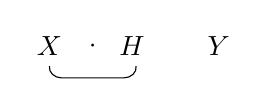
\begin{tikzpicture}[baseline]
\node at (0,0) {$X$};\node at (.55,0) {$\cdot$};\node at (1.05,0) {$H$};\node at (2.15,0) {$Y$};
\draw (0,-.25) to[out=-100,in=180] (.15,-.4) -- (.95,-.4) to[out=0,in=-80] (1.1,-.25);
\end{tikzpicture}}
\[
[X,Y]=0.
\]

Algèbre de Lie de $\unsure{\mathrm{SL}(2,k)}$ \hfill Car 2.
\[
\deleted{[X,H]=\lambda\unsure{L}}
\]
\[
\left\{\begin{aligned}
[H,X]&=\deleted{\unsure{2X}}\ 0\\
[H,Y]&=\deleted{\unsure{-2Y}}\ 0\\
[X,Y]&=H
\end{aligned}\right.
\qquad\mathfrak u
\]
Normalisateur de $k.Y=\mathfrak u$ est $k.Y+k.H=\unsure{\mathcal L|\mathfrak b}$

Normalisateur de $k.H=\unsure{\mathfrak h_\alpha|\mathfrak h}$ est $\mathfrak g$ \unsure{tt entier}

Algèbre de Lie de $\unsure{\mathrm{SPL}(2,k)|\mathrm{PGL}(2,k)}$
\[
\left\{\begin{aligned}
[H',X]&=X\\
[H',Y]&=-Y\\
[X,Y]&=0
\end{aligned}\right.
\]
Normalisateur de $k.Y$ est $\mathfrak g$

Normalisateur de
\margin{41}
\scanpage{45}
\uline{Formes extérieures types}

\margin{$E_0=\operatorname{Ext}(G_0)$\\$H_0=\operatorname{ad}(G_0)$\\$\Gamma_0=E.H$}

$G_0$ un groupe \unsure{s. simple} type (sur $\mathbb Z$), $\Gamma_0=\underline{\operatorname{Aut}}_{\mathbb Z}(G_0)$, \deleted{$\unsure{E=\Gamma/\Gamma^0}$} ou \deleted{$\unsure{E_0}$}.
\inserted{$E_0$ \unsure{sous-groupe} normalisant $T_0\subset B_0$}
$S$ schéma de base

$G$ forme de $G_0$ sur $S$, correspond à un principal homogène \deleted{$\unsure{Q_G}$}\inserted{$\unsure{Q_0}$} $\Gamma_S$, \deleted{\unsure{sous}}
\deleted{$\unsure{Q_G/E_0}$}\inserted{$\rho=\rho_G$}, principal homogène associé de groupe $E$, \deleted{qui} est \unsure{noté} par abus de langage l'élément correspondant de $H^1(S,E_0)$.

\deleted{\unsure{le principal} $\unsure{G_0^\rho}$}
$G_1=G_0^\rho$ déduit de $G_0$ en tordant par $\rho$ \inserted{[\unsure{par l'interméd.} \unsure{via} : $\unsure{\rho:E_0}$]} : une telle \deleted{groupe} forme sera dite \uline{forme extérieure type} associée à $\rho$.
[On dit que $G$ est une forme extérieure type s'il est \uline{isom.} à $G_{\unsure{1|0}}^\rho$, \deleted{$\unsure{G}$} \unsure{on a nécessairement} $\rho\simeq\rho_G$]

Si on part de $\rho$, [sans $G$], \uline{la donnée d'un $G$ et d'un isom} $\rho\xrightarrow[\sim]{\varphi}\rho_G$ \uline{``équivaut''} \uline{à la donnée d'un fibré principal homogène sous} $H_1=\unsure{H_0^\rho}$, la classification des objets $G$ à isom près :
[un isom de $(G,\varphi)$ et $(G',\varphi')$ étant donné par un isom $\psi:G\longrightarrow G'$ tel que l'isom correspondant $\rho_G\xrightarrow{\sim}\rho_{G'}$ soit compatible avec les deux $\rho_G$ et $\rho_{G'}$ \unsure{avec} $\varphi$ $\varphi'$ ; \uline{un tel automorphisme est dit intérieur}] \deleted{\unsure{revient}} \deleted{à classifier} est donnée par $H^1(S,\unsure{H_1})$. On a

\margin{Distinguer entre les deux \unsure{versions} avec $G_0$ et $H_0$, et avec $G_1$ et $H_1$ \unsure{-----}}
\margin{\unsure{Relier ici} la notion d'isom. \uline{intérieur} d'un \unsure{groupe}.}

\diagram{\begin{tikzcd}[ampersand replacement=\&,column sep=large]
H^1(S,\unsure{H_1}) \arrow[r] \& H^1(S,\Gamma) = \begin{array}{l}\text{ens des classes d'isom}\\\text{des formes de}\\G\text{ sur }S\end{array}\\
\begin{array}{l}\text{``ens des classes à}\\\text{isom près de ``formes}\\\deleted{\text{\unsure{extérieures}}}\ \text{intérieures relatives}\\\text{à }\rho\text{''}\end{array} \&
\end{tikzcd}}
\margin{44}
\scanpage{46}
\margin{45}
- \mspage{73} - \hfill n$^{\mathrm{o}}$ 239

\S\ 4. \uline{Prolongement de sections}. \uline{Faisceaux fins}

1. \uline{Sections d'un faisceau déduit d'un préfaisceau}.

Soient $(\mathcal F_U;\rho_{VU})$ un préfaisceau sur un espace $X$, $\mathcal F$ le faisceau qui s'en déduit. On a vu au \S\ 1, n$^{\mathrm{o}}$ 7 que, moyennant les conditions $(\mathrm{PF}_{\mathrm I}(U))$ et $(\mathrm{PF}_{\mathrm{II}}(U))$, supposées vérifiées pour tout $U\in\Phi$ \uline{toute} section de $\mathcal F$ au-dessus d'un ensemble $U\in\Phi$ est de la forme $x\longrightarrow\rho_{x,U}(f_U)$, où $f_U\in\mathcal F_U$ (\S\ 1, prop.14). Nous allons voir que dans certains cas la condition $(\mathrm{PF}_{\mathrm{II}}(U))$ à elle seule est suffisante pour qu'on puisse aboutir à cette conclusion :

PROPOSITION 1. - \uline{Soient} $X$ \uline{un espace topologique}, $(\mathcal F_U;\rho_{VU})$ \uline{un préfaisceau sur} $X$ \uline{relatif à l'ensemble} $\Phi$ \uline{de toutes les parties ouvertes de} $X$, $\mathcal F$ \uline{le faisceau déduit de ce préfaisceau}. \uline{Si} $U\in\Phi$ \uline{est un sous-espace paracompact de} $X$, \uline{et si la condition} $(\mathrm{PF}_{\mathrm{II}}(U))$ \uline{est satisfaite}, \uline{toute section de} $\mathcal F$ \uline{au-dessus de} $U$ \uline{est de la forme} $x\longrightarrow\rho_{x,U}(f_U)$.

Nous démontrerons d'abord le lemme suivant :

LEMME 1. - \uline{Soient} $Y$ \uline{un espace normal}, $(U_\alpha)_{\alpha\in A}$ \uline{un recouvrement ouvert localement fini de} $Y$. \uline{Pour tout couple d'indices} $\alpha,\beta$ \uline{et tout} $y\in U_\alpha\cap U_\beta$, \uline{supposons donné un voisinage ouvert} $V_{\alpha\beta}(y)$ \uline{de} $y$ \uline{contenu dans} $U_\alpha\cap U_\beta$. \uline{Alors}, \uline{il existe une application} $y\longrightarrow V(y)$ \uline{de} $Y$ \uline{dans l'ensemble des parties ouvertes de} $Y$, \uline{telle que pour tout} $y\in Y$, \uline{on ait} $y\in V(y)$, \uline{et que les conditions suivantes soient remplies} :

1) \uline{si} $y\in U_\alpha\cap U_\beta$, $V(y)\subset V_{\alpha\beta}(y)$ ;

2) \uline{si} $y',y''$ \uline{sont tels que} $V(y')\cap V(y'')\ne\phi$, \uline{il existe un} $\alpha$ \uline{tel que} $V(y')\cup V(y'')\subset U_\alpha$.

En effet, $(U_\alpha)$ étant un recouvrement localement fini et $Y$ étant
\scanpage{47}
\unsure{Le schéma suivant associé à} $G$ \unsure{est exact} de \unsure{groupes} sur $S$
\diagram{\begin{tikzcd}[ampersand replacement=\&]
e \arrow[r] \& \unsure{H_1^\rho} \arrow[r] \& \Gamma_1^\rho \arrow[r,dash] \& E_1^\rho \arrow[r,dash] \& e
\end{tikzcd}}
\[
\Gamma_1^\rho\simeq E_1^\rho.\unsure{H_1^\rho}
\]
qui permet d'écrire
\diagram{\begin{tikzcd}[ampersand replacement=\&,column sep=large]
H^0(S,E_1^\rho) \arrow[r] \& H^1(S,\unsure{H_1^\rho}) \arrow[r] \& H^1(S,\Gamma_1^\rho) \arrow[r] \arrow[d,equal] \& H^1(S,E^\rho)\\
\&\& H^1(S,\Gamma)\&
\end{tikzcd}}

\deleted{\unsure{On sait}}
A priori, l'application envisagée n'est pas injective. \deleted{\unsure{Ainsi}}\inserted{\unsure{Cependant}} l'ens des éléments de $H^1(S,\unsure{H_1^\rho})$ qui donnent l'élément neutre de $H^1(S,\Gamma_1^\rho)$ \deleted{\unsure{est celui qui}} est en correspondance biunivoque avec $H^0(S,E^\rho)/\operatorname{Im}H^0(S,\Gamma^\rho)$, est trivial puisque $\Gamma_1^\rho$ est un produit \unsure{semi-direct}.

Mais si $\xi\in H^1(S,\unsure{H_1^\rho})$, on peut utiliser $\xi$ pour tordre encore la situation, on trouve
\diagram{\begin{tikzcd}[ampersand replacement=\&,column sep=small]
e \arrow[r] \& (\unsure{H_1^\rho})^\xi \arrow[r] \& (\Gamma_1^\rho)^\xi \arrow[r] \arrow[d,equal] \& (E_1^\rho)^{\deleted{\unsure{\xi}}} \arrow[r] \& e\\
e \arrow[r] \& \operatorname{Ad}(G) \arrow[r,dash] \& \operatorname{Aut}(G) \arrow[r,dash] \& \operatorname{Ext}(G) \arrow[r] \& e
\end{tikzcd}}
et ici on est ramené à la question si tout automorphisme ext. de $G$ provient d'un automorphisme. Ce n'est pas du tout évident quand $G$ n'est \deleted{\unsure{automorphisme}} pas une forme extérieure type. [i.e. \deleted{\unsure{un groupe}} n'\unsure{a} pas de ss-groupe de Borel $\supset$ Tore maximal].

\margin{\figure{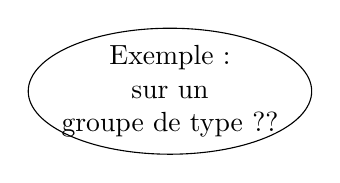
\begin{tikzpicture}\node[align=center] at (0,0) {\uline{Exemple} :\\\unsure{sur un}\\\unsure{groupe de type} ??};\draw (0,0) ellipse (1.8 and .8);\end{tikzpicture}}}
\margin{Faux sur $\mathbb R$ avec les formes \unsure{diverses} (\unsure{groupe unitaire}) : deux formes hermitiennes \unsure{opposées|voisines} donnant le \unsure{même} groupe algébrique sur $\mathbb R$ mais \uline{\unsure{ne sont pas}} isom.}
\margin{46}
\scanpage{48}
\margin{47}
- \mspage{83} - \hfill n$^{\mathrm{o}}$ 239

de toutes les parties fermées de $X$ contenues dans $U$.

*3) On voit de la même manière que si $X$ est une \uline{variété différentiable}, le faisceau $\mathcal F$ des \uline{germes de fonctions différentiables} sur $X$ est un faisceau mou d'anneaux.*

COROLLAIRE. - \uline{Si} $\mathcal A$ \uline{est un faisceau mou d'anneaux sur} $X$, \uline{tout faisceau quotient de} $\mathcal A$ \uline{est mou}.

En effet, soient $\mathcal B$ un anneau quotient de $\mathcal A$, $\varphi$ l'homomorphisme canonique de $\mathcal A$ sur $\mathcal B$ ; le corollaire résulte du fait que pour toute section $s$ de $\mathcal A$ au-dessus de $U\subset X$, $\varphi\circ s$ est une section de $\mathcal B$ au-dessus de $U$, et que l'on a $\varphi(1_x)=1_x$, $\varphi(0_x)=0_x$.

5. \uline{Partitions de l'unité dans les faisceaux mous d'anneaux}.

Soit $(s_\lambda)_{\lambda\in L}$ une famille de sections \uline{au-dessus de} $X$ d'un faisceau d'anneaux $\mathcal A$ (ou d'un faisceau de modules $\mathcal F$). On dit que la famille $(s_\lambda)$ est \uline{localement finie} si la famille $(\operatorname{Supp}(s_\lambda))_{\lambda\in L}$ de leurs supports est localement finie, autrement dit, si pour tout $x\in X$, il existe un voisinage $T$ de $x$ ne rencontrant qu'un nombre fini de supports des $s_\lambda$. Dans la somme $\sum_{\lambda\in L}s_\lambda(y)$ où $y\in T$ il n'y a qu'un nombre fini d'indices $\lambda$ (indépendants de $y$) tels que $s_\lambda(y)\ne0_y$, d'où résulte que l'application $x\longrightarrow\sum_{\lambda\in L}s_\lambda(x)$ est définie et continue dans $X$, et par suite est une \uline{section} de $\mathcal A$ au-dessus de $X$, que l'on note $\sum_{\lambda\in L}s_\lambda$.

Soit maintenant $\mathcal U=(U_\lambda)_{\lambda\in L}$ un recouvrement ouvert de $X$. Nous appellerons \uline{partition de l'unité subordonnée à} $\mathcal U$ \uline{dans} $\mathcal A$ toute famille \uline{localement finie} $(s_\lambda)_{\lambda\in L}$ de sections de $\mathcal A$ au-dessus de $X$ vérifiant les conditions suivantes :

$(\mathrm{PU}_{\mathrm I})$ \uline{Le support de} $s_\lambda$ \uline{est contenu dans} $U_\lambda$ \uline{pour tout} $\lambda\in L$.

$(\mathrm{PU}_{\mathrm{II}})$ \uline{On a} $\displaystyle\sum_{\lambda\in L}s_\lambda=1$.
\scanpage{49}
\diagram{\begin{tikzcd}[ampersand replacement=\&,column sep=small,row sep=large]
\text{Fibré des tores maximaux de }G\text{ est} \& P/N_1 \simeq Q/N'_1 \& {}=\mathcal C(G)\\
\text{--- Borel ---} \& P/B_1\simeq Q/B'_1 \& {}=\mathcal D(G)\\
\text{--- couples de Killing ---}\arrow[d,equal] \& P/T_1\simeq Q/T'_1\arrow[d,equal] \& {}=\mathcal C'(G)\arrow[u]\arrow[uu,bend right=50,"\text{fibré principal sous }W_1"']\\
\text{--- }\left\{\begin{array}{l}\text{Tores maximaux \unsure{piqués|pointés} de }G\\\text{Immersions intérieures }T_1\to G\end{array}\right\} \& P/T_1 \&
\end{tikzcd}}
\margin{fibré \deleted{\unsure{en fibres}} \unsure{sous} $B_1/T_1=\mathcal C(B_1)$ associé à un fibré principal \unsure{homogène} de gr $B_1$}

\uline{N.B.} Soit $T$ un tore \inserted{\uline{maximal de $G$}}, il y a correspondance biunivoque (\unsure{fonctorielle} $S'/S$) entre les ensembles suivants

a) L'ens des Borel contenant $T$

b) L'ens des isom $T_1-T$ qui sont intérieurs
\margin{$\left\}\unsure{P/T_1}\simeq P'/T'_1\right.$}

\deleted{\unsure{Puis qui}}\unsure{plus}, \deleted{\unsure{on a les conditions}} \inserted{la \unsure{définition} est \unsure{généralisée} par b) :} \deleted{il existe une \unsure{application}}

b') L'ens des isom $T_1\longrightarrow T$ qui sont ``géom$^{\mathrm t}$ \unsure{extérieurs|intérieurs}''
\margin{$\left\}P'/T_1\right.$}
\deleted{\unsure{Autrement dit}} Il existe une projection de b') sur b).

\margin{$W_1$ et $W$ sont \unsure{commutants} l'un de l'autre \unsure{dans cet ens} $P_1$ \unsure{supposé} \unsure{principal} \unsure{lorsque les deux schémas sont} $\ne\phi$]}

De plus les conditions suivantes sur $T$ sont équivalentes

$\alpha$) $T$ est contenu dans un Borel

$\beta$) Il existe un isom intérieur $T_1-T$

$\gamma$) Il existe un isom \unsure{extérieur} $T_1-T$

On dit alors que $T$ est un ``Tore de \unsure{Killing}''. Pour qu'il existe, il f. et s. que $G$ soit isomorphe à une forme extérieure type.

L'image inverse de $\xi\in H^1(S,G_1)$ dans $H^1(S,B_1)$ est en correspondance biunivoque avec l'ens des sous-groupes de Borel de $G$, modulo automorphismes intérieurs ; Il est non vide [i.e. on peut restreindre le groupe structural à $B_1$] dès qu'il existe un sous-groupe de Borel; dans ce cas, il est réduit à un élément : \unsure{on dit} ces deux sous-groupes de Borel de $G$ sont tous conjugués. \deleted{\unsure{Cela est}}

\margin{On n'a \unsure{besoin} que $G_1$ soit une forme extérieure type, mais seulement qu'il y ait un ss-groupe de Borel}

\figure{\begin{tikzpicture}\node[draw,align=left,text width=12cm] {[\uline{Question} ? Cette \deleted{\unsure{condition est vérifiée}} \inserted{\figure{\begin{tikzpicture}[baseline=(d.base)]\node (d) {\unsure{dernière}};\draw (d.center) ellipse (0.85cm and 0.24cm);\end{tikzpicture}} condition} \unsure{est-elle} tjrs \unsure{vérifiée} ? Si $S$ est local ?]};\end{tikzpicture}}
\margin{$\times$}
\margin{48}
\scanpage{50}
\margin{49}
- \mspage{74} - \hfill n$^{\mathrm{o}}$ 269

PROPOSITION 3 - \uline{Soit} $\Phi$ \uline{une forme} $\epsilon$-\uline{hermitienne vérifiant} (T) (resp. \uline{la forme bilinéaire associée à une forme quadratique non dégénérée} $Q$). \uline{Soient} $F_1$ \uline{et} $F_2$ \uline{deux sous-espaces totalement isotropes} (resp. \uline{totalement singuliers}) \uline{maximaux de} $E$, \uline{l'un des deux étant de dimension finie}. \uline{Posons} $F=F_1\cap F_2$. \uline{Soit} $S_i$ $(i=1,2)$ \uline{un supplémentaire de} $F$ \uline{dans} $F_i$ ; \uline{posons} $S=S_1+S_2$. \uline{Il existe alors deux sous espaces} $G$ \uline{et} $H$ \uline{de} $E$ \uline{tels que}

a) \uline{Les sous-espaces} $G+F$, $S$ \uline{et} $H$ \uline{sont non isotropes et deux à deux orthogonaux},

b) $E$ \uline{est somme directe de} $F,S,G$ \uline{et} $H$,

c) \uline{Il n'y a aucun vecteur isotrope} (resp. \uline{singulier}) \uline{non nul dans} $H$,

d) $G$ \uline{est totalement isotrope} (resp. \uline{totalement singulier}).

\uline{De plus}, $F_1$ \uline{et} $F_2$ \uline{sont tous deux de dimensions finies et on a}
\[
\begin{gathered}\dim F_1=\dim F_2,\quad\dim G=\dim F,\quad\dim S_1=\dim S_2,\quad\operatorname{codim}H={}\\=2\dim F_1.\end{gathered}
\]

Remarquons d'abord que, si $N$ est un sous espace totalement isotrope (resp. totalement singulier) maximal, alors tout vecteur isotrope (resp. singulier) $x$ orthogonal à $N$ est un élément de $N$, car sinon $N+Ax$ contredirait le caractère maximal de $N$.
Donc si, pour $i=1,2$, $x_i$ est un vecteur isotrope (resp. singulier) de $F_i^{\mathrm o}$, on a $x_i\in F_i$. D'autre part, si $y$ est un élément de $S_1$ orthogonal à $S_2$, il est orthogonal à $F_1$ puisque $F_1$ est totalement isotrope, donc à $F$, et par suite à $F_2=S_2+F$. Comme $y$ est isotrope (resp. singulier) et qu'il est orthogonal à $F_2$, on
\scanpage{51}
L'image inverse de $\xi$ dans $H^1(S,N_1)$ est en correspondance biunivoque avec l'ens des Tores maximaux de $G$, modulo automorphismes intérieurs. En particulier, il est non vide \deleted{\unsure{ssi}} i.e. on peut restreindre le groupe structural à $N_1$, ssi il existe un tore maximal; s'il en est ainsi, alors il est réduit à un élément ssi tous les tores maximaux sont conjugués, [ce qui n'est vrai que exceptionnellement dans des situations ``arithmétiques''].

\margin{Vaut \deleted{\unsure{pour}} \unsure{sans supposer} \unsure{seulement} que $G_1$ \unsure{ait un tore maximal}.}
\margin{\figure{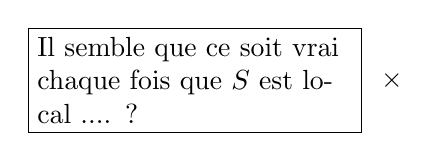
\begin{tikzpicture}\node[draw,align=left,text width=4cm] {Il semble que ce soit vrai chaque fois que $S$ est local .... ?};\node at (2.5,0) {$\times$};\end{tikzpicture}}}

\margin{\deleted{\unsure{donc}} Si $S$ local, \deleted{$T_1\ \unsure{est déployé}$}, $N_1$ produit \unsure{semi-direct} de $W_1=W_0$ \unsure{et} $T_1$, on a
\diagram{\begin{tikzcd}[ampersand replacement=\&]H^1(S,N_1)\arrow[r,"\text{surj}"]\&H^1(S,W_0)\end{tikzcd}}.
\unsure{Le résultat} \deleted{\unsure{précédent}} \unsure{se démontre} \deleted{\unsure{ainsi}} si on est \unsure{sur un} \unsure{anneau} \unsure{de} \deleted{\unsure{Tores}} \unsure{locaux}; exprimer qu'un élément de $H^1(S,W_0)$ donne \unsure{l'image} $\xi$ \deleted{\unsure{neutre}}.}
\margin{\figure{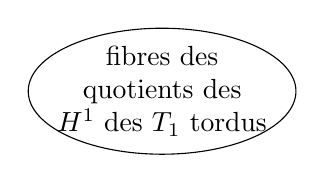
\begin{tikzpicture}\node[align=center] at (0,0) {fibres des\\quotients des\\$H^1$ des $T_1$ tordus};\draw (0,0) ellipse (1.7 and .8);\end{tikzpicture}}}

L'image inverse de $\xi$ dans $H^1(S,\unsure{\overline N_1})$ est en correspondance biunivoque avec l'ens des couples $(T\subset B)$ de Killing dans $G$, modulo aut. extérieurs; Donc il est non vide ssi il existe un tel couple, ou encore s'il existe un Tore \deleted{privilégié} de Chevalley, ou encore un Borel de Chevalley, \inserted{[donc exceptionnel \unsure{dans des cas arithmétiques}];} et \deleted{\unsure{dans ce cas}} s'il en est ainsi, alors l'ens est réduit à un élément ssi \deleted{\unsure{deux}} couples de Killing de $G$ sont conjugués.
[et il est probable que cette condition soit vérifiée sur tt anneau local; c'est évidemment le cas si on suppose de plus $T_1$ trivial \inserted{[i.e. $\rho=0$]}, par le lemme de \unsure{Bru---}]

\margin{Question équivalente : les \unsure{ss-groupes} \unsure{de} \deleted{\unsure{paraboliques}} Borel sont conjugués ? \unsure{Dans un Tore} \unsure{maximal} d'un \uline{Borel $B$} \unsure{sont ils toujours} conjugués \unsure{dans $G$} \uline{dans $B$}}
\margin{50}
\scanpage{52}
\margin{51}
- \mspage{73} - \hfill n$^{\mathrm{o}}$ 269

$\dim G<\dim F$, la restriction de $\Phi$ à $F\times G$ est dégénérée, et donc, comme $G\cap F^{\mathrm o}$ est nul, $F\cap G^{\mathrm o}$ est non nul. Si l'on avait alors $G+F^{\mathrm o}\supset G^{\mathrm o}$, on en déduirait, en prenant les orthogonaux et en remarquant que $F=F^{\mathrm{oo}}$ et que $G=G^{\mathrm{oo}}$, que $G^{\mathrm o}\cap F\subset G$, d'où $G^{\mathrm o}\cap F\subset G\cap F\subset G\cap F^{\mathrm o}=\{0\}$, ce qui est impossible. Il existe alors un élément $x$ de $G^{\mathrm o}$ tel que $x\notin G+F^{\mathrm o}$ ; comme $G\subset G^{\mathrm o}$ et $F\subset F^{\mathrm o}$, on peut ajouter à $x$ un vecteur de $G^{\mathrm o}\cap F$ sans modifier ces propriétés ; comme $G^{\mathrm o}\cap F$ est totalement isotrope (resp. totalement singulier) et $\ne\{0\}$, le lemme montre qu'on peut choisir $x$ isotrope (resp. singulier). Alors le sous espace $G'=G+Ax$ est de dimension $s+1$, et est totalement isotrope (resp. totalement singulier) ; de plus on a $G'\cap F^{\mathrm o}=\{0\}$ car, si $y=z+ax$ $(z\in G,a\in A)$ est dans $F^{\mathrm o}$, on a $a=0$ car sinon $x\in F^{\mathrm o}+G$ contrairement au choix de $x$, d'où $y=z\in G\cap F^{\mathrm o}=\{0\}$ et $y=0$. Par conséquent le sous espace $G'$ répond à la question.

COROLLAIRE - \uline{Si} $F$ \uline{est un sous-espace totalement isotrope} (resp. \uline{totalement singulier}) \uline{de dimension} $r$, \uline{il existe un sous espace totalement isotrope} (resp. \uline{totalement singulier}) $F'$ \uline{de dimension} $r$ \uline{tel que} $F\cap F'=\{0\}$ \uline{et que} $F+F'$ \uline{soit non isotrope}.

Il suffit de faire $G=\{0\}$ dans la prop. 2,b).

\uline{Remarque}. Dans les conditions du corollaire, $E$ est somme directe de $F+F'$ et de l'orthogonal de $F+F'$. On a donc une décomposition de Witt de $E$. D'après la prop.2,a), il existe des bases de $F$ et $F'$ telles que, dans la matrice (1) de $\Phi$, le bloc $\unsure{\mathcal U|\mathcal A}$ soit la matrice unité $\unsure{\underline{1}_r}$.
\scanpage{53}
\uline{Th.} Conditions équivalentes sur $\xi\in H^1(S,H_1)$, définissant $G=G_1^\xi$.
\textcircled{i}  $\xi\in\operatorname{Im}H^1(S,T_1)$ dans $H^1(S,H_1)$

(i') $\overline\xi\in\operatorname{Im}H^1(S,T'_1)$ dans $H^1(S,\Gamma_1)$ / ou $\overline\xi_0\in\operatorname{Im}H^1(S,T'_0)$ dans $H^1(S,\unsure{\Gamma'_0})$

(i'') $\overline\xi\in\operatorname{Im}H^1(S,T_1)$ dans $H^1(S,\Gamma_1)$ / ou $\overline\xi_0$

\textcircled{ii} Il existe un couple de Killing dans $G$, i.e. un Borel $\supset$ Tore max.

[\deleted{\textcircled{iii}} Il existe un \deleted{Tore maximal \unsure{intérieur isomorphe}} \deleted{\unsure{contenant de}} Tore maximal de $G$, \deleted{\unsure{isom. à} $T_1$} provenant \deleted{\unsure{d'un}} d'une immersion \uuline{extérieure} $T_1-G$]

\textcircled{iii'} Il existe une \uline{immersion intérieure} de $T_1$ dans $G$.

\margin{De plus, si $T$ est un Tore maximal, conditions équival. :
\diagram{\begin{tikzcd}[ampersand replacement=\&,column sep=small]
\text{a) }\exists\text{ Borel}\supset T \arrow[dr,Rightarrow] \& \text{b) }\exists\text{ isom }T_1\to T\ \text{extérieur}\\
\&\text{c) }\exists\text{ isom }T_1\to T\ \text{intérieur}
\end{tikzcd}}}

\deleted{\uline{Dém}}
\diagram{\begin{tikzcd}[ampersand replacement=\&,column sep=small,row sep=huge]
(iii')\arrow[r,Leftrightarrow]\arrow[d,Rightarrow,"\text{triv}"'] \& (i)\arrow[r,Leftrightarrow]\deleted{\arrow[dl,Rightarrow]} \& (i')\arrow[r,Leftrightarrow]\deleted{\arrow[d,Rightarrow,"\unsure{triv}"']} \& \deleted{(ii)}\arrow[r,Leftrightarrow] \& \deleted{\unsure{(iii')}}\\
(iii)\arrow[rr,Leftrightarrow] \&\& (i'')\arrow[u,Rightarrow,"\text{triv}"]\deleted{\arrow[ur,Rightarrow]} \& \&
\end{tikzcd}}
\deleted{\unsure{uniquement des lois de conjugaison}.}
\deleted{Car le centralisateur de $T_1$ en $\Gamma_1$ est $T_1$}

\uline{N.B.} Supposons que $T_1$ soit $\simeq G_m^r$ (\uline{\unsure{cas d'un anneau}} \uline{local}]. Alors \uline{$\forall$} tore $T\subset G$ qui est $\simeq T_1$, est \deleted{un tore de \unsure{Borel type}} contenu dans un Borel, \deleted{\unsure{donc}} i.e. il existe un isom \uline{intérieur} de $T_1$ sur $T$. \deleted{La \unsure{preuve}}\inserted{En effet}, \deleted{\unsure{étant local}} les \inserted{\unsure{schéma des}} isom \uline{intérieurs} de $T_1$ dans $T$ forment un sous-schéma de $\underline{\operatorname{Isom}}_S(T_1,T)\simeq(\mathbb Z^{r^2})_S$, qui est fini étale sur $S$ de groupe $W$, donc \unsure{l'un est une réunion de composantes}. \uline{Or} D., \unsure{en un}

\margin{Et si $\operatorname{Pic}(S)=e$, il existe un isom de \unsure{Tch} de $G_0$ sur $G$, transformant $T_0$ en $T$.}
\margin{52}
\scanpage{54}
\margin{53}
- \mspage{68} - \hfill n$^{\mathrm{o}}$ 269

Un vecteur isotrope n'est autre qu'un vecteur orthogonal à soi-même. Dire qu'un sous-module $F$ est isotrope signifie que $F\cap F^{\mathrm o}\ne\{0\}$, ou encore que la restriction de $\Phi$ à $F$ est dégénérée; un sous-module \uline{non isotrope} $G$ de $E$ est donc un sous module tel que la restriction de $\Phi$ à $G$ est non dégénérée. Pour qu'un sous module $F$ de $E$ soit totalement isotrope, il faut et il suffit que l'on ait $F\subset F^{\mathrm o}$. Si $F$ est un sous-module totalement isotrope de $E$, il en est de même de tout sous-module $F'$ contenu dans $F$. La somme d'une famille de sous-modules totalement isotropes et orthogonaux deux à deux est un sous-module totalement isotrope.
L'ensemble des sous-modules totalement isotropes de $E$, ordonné par inclusion, est évidemment inductif ; il en résulte que tout sous-module totalement isotrope est contenu dans un \uline{sous-module totalement dégénéré maximal}.

PROPOSITION 1 - \uline{On suppose que} $A$ \uline{est un corps}. \uline{Soit} $F$ \uline{un sous-espace non isotrope de dimension finie de} $E$ ; \uline{alors} $E$ \uline{est somme directe de} $F$ \uline{et de} $F^{\mathrm o}$. \uline{Si} $E$ \uline{est somme directe d'une famille} $(E_i)_{i\in I}$ \uline{de sous espaces deux à deux orthogonaux}, \uline{pour que} $\Phi$ \uline{soit non dégénérée}, \uline{il faut et il suffit que chacun des} $E_i$ \uline{soit non isotrope dans ces conditions l'orthogonal de} $E_i$ \uline{est le sous-espace} $\sum_{j\ne i}E_j$.

En effet, comme la restriction $\Phi'$ de $\Phi$ à $F$ est non dégénérée par hypothèse, l'application $d_{\Phi'}$ de $F$ dans son dual $F^*$ associée à droite à $\Phi'$ est injective donc bijective puisque $F$ et $F^*$ sont deux espaces de même dimension finie. Par suite, pour tout $y\in E$,
\scanpage{55}
\uline{Question 1} Supposons que \deleted{$G$ ait un} $T$ qui \deleted{est}\inserted{soit} $\simeq T_1$, alors ce $T$ est-il contenu dans un Borel, i.e. est-ce qu'il existe un isom \uuline{intérieur} $T_1-\unsure{T_\rho|T}$ ??
J'en doute.

\uline{Question 2} Supposons que \deleted{$T_1$ soit isom. à} $G$ ait un \deleted{\unsure{groupe}} tore maximal $T$ contenu dans un Borel. S'ensuit-il que $G\simeq G_1$ ? \deleted{\unsure{Je ne sais}} \deleted{\unsure{si on a} $\rho$ \unsure{trivial}} C'est le cas si $\operatorname{Pic}(S)=0$ \inserted{\figure{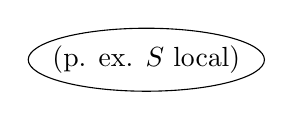
\begin{tikzpicture}\node at (0,0) {(p. ex. $S$ local)};\draw (0,0) ellipse (1.5 and .4);\end{tikzpicture}}} et si $\rho$ \deleted{\unsure{est}} est trivial. Est-ce vrai sur un corps $k$ ($\rho$ non trivial) ??

\margin{N.B. on utilise que le normalisateur de $(B_0,T_0)$ dans $\Gamma_0$ est $T'_0$ \deleted{\unsure{mais} $\unsure{T_0}$} \deleted{\illegible{3}} \unsure{alors} \unsure{dans le cas} \unsure{d'un groupe} \unsure{on a} \deleted{\unsure{un groupe}} \unsure{``} $\unsure{W}$ \unsure{''} \deleted{\illegible{2}} \unsure{extérieure}.}

\deleted{Par exemple $k=\mathbb R$, groupe unitaire.} C'est encore vrai si $k$ est un \uline{corps de Tsen}
[$H^1(k,T)=0$ pour \uline{$\forall$} tore sur $k$]. Que se passe-t-il pour $k=\mathbb R$, \deleted{\unsure{lorsque}} $G_1,G$ groupes \inserted{projectifs} unitaires spécial à deux variables ???

\margin{Dans ce cas on aura $=$ $\xi=e$}

\deleted{\unsure{\S}}
\uline{Question 3} Supposons qu'il existe un sous-groupe de Borel $B$ de $G$ \inserted{\unsure{localement conjugué} \unsure{au} $G_1:B_1$}, Alors peut-on réduire le groupe structural \deleted{à} de $G_1$ à $T_1$, et $=$ est-il vrai que \deleted{\unsure{l'on}} l'on peut trouver un sous-groupe
\margin{54}
\scanpage{56}
\margin{55}
- \mspage{75} -
\hfill n°269

a $y\in S_1\cap F_2=S_1\cap F_1\cap F_2=S_1\cap F=\{0\}$. On a donc $S_1\cap S_2^{\mathrm o}=\{0\}$, et de même $S_2\cap S_1^{\mathrm o}=\{0\}$. Comme l'un des deux sous-espaces $F_1,F_2$, par exemple $F_1$, est de dimension finie, $S_1$ est de dimension finie, donc $S_1^{\mathrm o}$ est de codimension finie, et par conséquent $S_2$ est de dimension finie puisque $S_2\cap S_1^{\mathrm o}=\{0\}$; de plus ceci montre que l'on a $\dim S_2\leq\operatorname{codim}S_1^{\mathrm o}=\dim S_1$ ; de même $\dim S_1\leq\dim S_2$, d'où $\dim S_1=\dim S_2$. La prop. 2,a) montre alors que $S=S_1+S_2$ est non isotrope.

Ceci étant, l'orthogonal $N$ de $S$ est non isotrope (cor. de la prop.1) et contient $F$. Le cor. à la prop.2 montre donc qu'il existe un sous espace $G$ totalement isotrope (resp. totalement singulier) de $N$ tel que $\dim G=\dim F$, que $G\cap F=\{0\}$ et que $G+F$ soit non dégénéré. Ainsi d) est vérifiée par $G$. On satisfera alors à a) et b) en prenant pour $H$ l'orthogonal de $G+F$ dans $N$. Quant à c), l'on remarque que, comme $H$ est orthogonal à $F_1=S_1+F$, il n'y a aucun vecteur isotrope (resp. singulier) non nul dans $H$ en vertu de ce qui a été remarqué au début de la démonstration et du fait que $H\cap F_1=\{0\}$. Enfin les assertions relatives aux dimensions ont été démontrées en cours de route, ou s'en déduisent trivialement.

COROLLAIRE 1 - \uline{Les hypothèses étant celles de la prop.3, deux sous-espaces totalement isotropes} (resp. \uline{totalement singuliers}) \uline{maximaux de dimensions finies ont même dimension. Pour tout sous-espace totalement isotrope} (resp. \uline{totalement singulier}) \uline{maximal} $F$ \uline{de dimension finie, il en existe un autre} $F'$ \uline{tel que} $F\cap F'=\{0\}$, \uline{et dans ces conditions} $F+F'$ \uline{est non isotrope.}
\scanpage{57}
$H^1(S,T_1)$ \unsure{classification des formes intérieures munies} d'un couple de Killing.

[N.B. si $G$ est une forme intérieure, \unsure{alors} deux couples de Killing \inserted{$(T,B),(T',B')$} dans $G$ définissent le $=$ élément de $H^1(S,T_1)$ ssi ils sont conjugués par un \unsure{aut.} intérieur. Car \unsure{à priori leur} \unsure{différence par une certaine classe} dans $H^1(S,\unsure{\overline B|\overline T})$ est \unsure{nulle|valable} --- si $T=T'$, c'est la classe \inserted{mod $\unsure{D}$} de l'unique $\sigma\in W(T)$ qui transforme $B$ en $B'$; si $B'$ est l'opposé de $B$ rel. à $T$, alors le $\sigma$ en question est \deleted{\unsure{donné par}} \unsure{l'image} \inserted{\unsure{can}} \unsure{d'un} élément \unsure{connu} de $H^1(S,T)$]

\margin{$H^1(S,T)\mathbin{-}H^1(S,B)$}

La question de savoir si deux couples de Killing dans un $=$ $G$ sont tjrs conjugués, \unsure{équivaut} donc à celle de savoir si $H^1(S,T_1)\mathbin{-}H^1(S,G_1)$ est tjrs injective. Pour un contre-exemple, il suffit de montrer que $H^1(S,T_1)\mathbin{-}H^1(S,N_1)$ n'est pas tjrs injective. Or deux \unsure{élémts} de $H^1(S,T_1)$ ont la $=$ image dans $H^1(S,N_1)$ ssi ils sont conjugués par $H^0(S,W_1)$ opérant de façon évidente. Je prendrai \unsure{$G$ pour} $G_0=\unsure{GP|GL}(2)$, avec $E=\mathbb Z/2\mathbb Z$, $W_0=\mathbb Z/2\mathbb Z$ est commutatif, \deleted{\unsure{donc} $\unsure{W_1=W_0}$ \unsure{comme}} $E$ y opère trivialt (il n'a pas le choix!) donc $W_0=W_1$, qui opère par symétrie sur $T_1$.
\margin{56}
\scanpage{58}
- \mspage{59} -
\hfill n°269

voit que les formules
\[
(3)\qquad f(x)=f_1(x)-if_1(j(x))
\]
\[
(4)\qquad f(x)=f_2(j(x))+if_2(x)
\]
($x\in E$, $f\in E^*$, $f_1,f_2\in(E_0)^*$) établissent deux correspondances biunivoques entre $E^*$ et $(E_0)^*$.

3 - \uline{Formes bilinéaires associées à une forme hermitienne.}

Nous supposons encore ici que l'anneau $A$ est l'\uline{extension quadratique} $A=K(i)$ (où $i^2=-1$) d'un anneau commutatif $K$, et que $J$ est l'automorphisme $\lambda+i\mu\longrightarrow\lambda-i\mu$ de $A$ ($\lambda,\mu\in K$). Soient $E$ et $E'$ deux $A$-modules, $E_0$ et $E'_0$ les $K$-modules sous-jacents à $E$ et $E'$, $j$ et $j'$ les automorphismes $x\longrightarrow ix$ et $x'\longrightarrow ix'$ de $E$ et $E'$ (cf.n°2). Une forme $K$-bilinéaire $f$ sur $E_0\times E'_0$ sera dite \uline{invariante} par $j$ et $j'$ si l'on a
\[
(5)\qquad f(j(x),j'(x'))=f(x,x')
\]
pour $x\in E_0$ et $x'\in E'_0$. Remplaçant $x$ par $j(x)$, on voit que cette condition équivaut à
\[
(6)\qquad f(x,j'(x'))=-f(j(x),x')
\]
pour tous $x\in E_0$ et $x'\in E'_0$.

PROPOSITION 1 - \uline{Soit} $\Phi_1$ (resp. $\Phi_2$) \uline{une forme} $K$-\uline{bilinéaire sur} $E_0\times E'_0$ \uline{invariante par} $j$ \uline{et} $j'$. \uline{L'application qui à} $\Phi_1$ (resp. $\Phi_2$) \uline{fait correspondre l'application} $\Phi$ \uline{de} $E\times E'$ \uline{dans} $A$ \uline{définie par}
\[
(7)\qquad\Phi(x,x')=\Phi_1(x,x')+i\Phi_1(x,j(x'))
\]
\[
(\text{resp.}\quad(8)\qquad\Phi(x,x')=-\Phi_2(x,j(x'))+i\Phi_2(x,x')\ )
\]
($x,x'\in E$), \uline{est un isomorphisme du} $K$-\uline{espace vectoriel des formes} $K$-\uline{bilinéaires sur} $E_0\times E'_0$ \uline{invariantes par} $j$ \uline{et} $j'$ \uline{sur le}
\margin{57}
\scanpage{59}
\diagram{
\[
\begin{array}{ccc}
\begin{gathered}\text{\unsure{forme extérieure}}\\G_1\ \text{\unsure{donnée}}\end{gathered}&
\left\{\begin{gathered}
\begin{tikzcd}[ampersand replacement=\&,row sep=large]
{H^1(S,G_1)\longrightarrow H^1(S,\Gamma_1)\quad\text{injectif ?}}\arrow[d,Rightarrow]\\
{\begin{gathered}\deleted{\unsure{H^1}}\\\underline{\operatorname{Aut}}(G)\longrightarrow\underline{\operatorname{Ext}}(G)\quad\text{admet tjrs}\\\text{une section}\end{gathered}}\arrow[d,Leftrightarrow]\\
{\operatorname{Aut}(G)\longrightarrow\operatorname{Ext}(G)\quad\text{tjrs surjectif}}
\end{tikzcd}
\end{gathered}\right\}&
\begin{gathered}\text{Non}\\\text{faux en général sur un corps}\\\text{vrai pour les formes}\\\text{intérieures}\quad\rho=0\\\text{ou sur les anneaux}\\\text{de Tsen}\end{gathered}
\end{array}
\]
}

\diagram{
\[
\begin{array}{cc}
\left.\begin{gathered}
\begin{tikzcd}[ampersand replacement=\&,row sep=large]
{H^1(S,B_1)\longrightarrow H^1(S,G_1)\quad\text{injectif}}\arrow[d,Leftrightarrow]\\
{\begin{gathered}\text{Deux sous-groupes de Borel \inserted{\figure{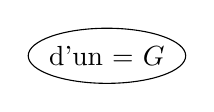
\begin{tikzpicture}\node at (0,0) {\uline{d'un} $=$ $G$};\draw (0,0) ellipse (1 and .35);\end{tikzpicture}}}}\\\text{tjrs conjugués}\end{gathered}}\arrow[d,Leftrightarrow]\\
{\begin{gathered}\text{Pour \uuline{tt.}}\ G\ \text{et}\ B,\quad\deleted{\text{le noyau de}}\\H^1(S,B)\longrightarrow H^1(S,G)\quad\deleted{\text{est injectif}}\end{gathered}}\arrow[d,Leftrightarrow]\\
{\begin{gathered}\text{Pour tt}\ G,\ \text{et}\ B,\quad\deleted{\text{le noyau de}}\\H^1(S,B)\mathbin{-}H^1(S,G)\quad\text{est \unsure{bijectif|injectif}}\end{gathered}}
\end{tikzcd}
\end{gathered}\right\}&
\begin{gathered}-\\\text{vrai pour les formes}\\\text{intérieures}\ (\rho=0)\\\text{ou sur les anneaux}\\\text{de Tsen.}\end{gathered}
\end{array}
\]
}

\margin{\unsure{d'un cas} \unsure{la} $=$ \unsure{chose pour} tt \unsure{extension de} $S$ \inserted{(ou $S'$ \uuline{local})} \unsure{la même chose} est équivalent à dire que $G\longrightarrow G/B$ est fibré \uline{localement trivial}.}

\diagram{
\[
\begin{array}{cc}
\left.\begin{gathered}
\begin{tikzcd}[ampersand replacement=\&,row sep=large]
{H^1(S,N_1)\mathbin{-}H^1(S,G_1)\quad\text{injectif}}\arrow[d,Rightarrow]\\
{\begin{gathered}\text{Deux sous groupes de Cartan du $=$}\ G\\\text{tjrs conjugués}\end{gathered}}\arrow[d,Leftrightarrow]\\
{\begin{gathered}\text{Pour tt.}\ G\ \text{et}\ T,\ \text{le noyau de}\\H^1(S,N(T))\mathbin{-}H^1(S,G)\\\text{trivial}\end{gathered}}\arrow[d,Leftrightarrow]\\
{\begin{gathered}\rule{4cm}{0.3pt}\\\hspace{1cm}\rule{2cm}{0.3pt}\quad\text{injectif}\end{gathered}}
\end{tikzcd}
\end{gathered}\right\}&
\begin{gathered}\deleted{\text{\unsure{Souvent}}}\ \text{faux déjà dans}\\\text{les corps \unsure{non}}\\\text{\unsure{p-adiques} : \unsure{leurs}}\\\text{\unsure{clôtures parfaites},}\\\text{$=$ pour les formes}\\\deleted{\unsure{R}}\ \text{intérieures, .....}\end{gathered}
\end{array}
\]
}
\margin{58}
\scanpage{60}
- \mspage{60} -
\hfill n°269

$K$-\uline{espace vectoriel des formes sesquilinéaires sur} $E\times E'$. \uline{Si l'on a de plus} $E=E'$, \uline{pour que} $\Phi$ \uline{soit hermitienne, il faut et il suffit que} $\Phi_1$ \uline{soit symétrique} (resp. \uline{que} $\Phi_2$ \uline{soit antisymétrique}).
\margin{\unsure{''}}

En effet toute application $\Phi$ de $E\times E'$ dans $A$ s'écrit, d'une manière et d'une seule, sous la forme $\Phi=\Phi_1+i\Phi_2$, où $\Phi_1$ et $\Phi_2$ sont des applications de $E\times E'$ dans $K$. Pour que l'application partielle $x\longrightarrow\Phi(x,x')$ soit $A$-linéaire, il faut et il suffit, d'après la formule (\unsure{5|3}) (resp. (4)) du n°2, que $\Phi_1$ (resp. $\Phi_2$) soit $K$-linéaire en $x$ et que l'on ait
\[
(9)\qquad\Phi(x,x')=\Phi_1(x,x')-i\Phi_1(j(x),x')
\]
\[
(\text{resp.}\quad(10)\qquad\Phi(x,x')=\Phi_2(j(x),x')+i\Phi_2(x,x')).
\]
De même, pour que $\overline{\Phi(x,x')}$ soit $A$-linéaire en $x'$, il faut et il suffit que $\Phi_1$ (resp. $\Phi_2$) soit $K$-linéaire en $x'$ et que l'on ait
\[
(11)\qquad\Phi(x,x')=\Phi_1(x,x')+i\Phi_1(x,j'(x'))
\]
\[
(\text{resp.}\quad(12)\qquad\Phi(x,x')=\Phi_2(x,j'(x'))+i\Phi_2(x,x')\ ).
\]
Il en résulte immédiatement que, pour que $\Phi$ soit sesquilinéaire, il faut et il suffit qu'elle s'écrive sous l'une ou l'autre des formes (9) et (11) (resp. 10) et (12)) avec $\Phi_1$ (resp. $\Phi_2$) $K$-bilinéaire invariante par $j$ et $j'$.

Il résulte de ceci que, pour qu'une forme sesquilinéaire $\Phi=\Phi_1+i\Phi_2$ soit nulle, il faut et il suffit que $\Phi_1$ (resp. $\Phi_2$) soit nulle. Or, si $E=E'$, on a
\[
\Phi(y,x)=\Phi_1(y,x)+i\Phi_2(y,x)\quad\text{et}\quad\overline{\Phi(x,y)}=\Phi_1(x,y)-i\Phi_2(x,y)\ ;
\]
pour que ces deux expressions soient égales, autrement dit pour
\margin{59}
\scanpage{61}
Formes quadratiques

bilinéaires \unsure{symm}

etc
\margin{60}
\scanpage{62}
\deleted{\diagram{
\begin{tikzcd}[ampersand replacement=\&,column sep=large,row sep=large,execute at end picture={
\draw ([xshift=-6pt,yshift=5pt]a.north west)--([xshift=-13pt,yshift=5pt]a.north west)--([xshift=-13pt,yshift=-5pt]b.south west)--([xshift=-6pt,yshift=-5pt]b.south west);
\draw ([xshift=6pt,yshift=5pt]a.north east)--([xshift=13pt,yshift=5pt]a.north east)--([xshift=13pt,yshift=-5pt]b.south east)--([xshift=6pt,yshift=-5pt]b.south east);
\draw ([xshift=6pt,yshift=5pt]c.north east)--([xshift=13pt,yshift=5pt]c.north east)--([xshift=13pt,yshift=-5pt]d.south east)--([xshift=6pt,yshift=-5pt]d.south east);
}]
|[alias=a]| {\text{Spéc Bil hyp}}\arrow[r]\arrow[d]\&{\text{Bil hyp.}}\arrow[d]\arrow[ddr]\&|[alias=c]|{\text{Quad \unsure{unimod}}}\arrow[d]\arrow[dl]\arrow[ddl,"{\deleted{\unsure{unimod}}}"',bend right=12]\\
|[alias=b]|{\text{Spéc. Bil unimod}}\arrow[r]\&{\text{Bil unimod}}\arrow[d]\&|[alias=d]|{\text{Quad hyp.}\deleted{\unsure{unimod}}}\arrow[d]\arrow[dl]\\
\&{\text{Bil}}\arrow[r,shift left]\arrow[ddr]\&{\text{Quad}}\arrow[l,shift left]\arrow[dd]\\
\&{\deleted{\text{Mod}}}\arrow[dr]\&\\
\&\&{\text{Mod}}
\end{tikzcd}
}}

\deleted{\diagram{
\begin{tikzcd}[ampersand replacement=\&,row sep=large]
{\text{Spéc Bil hyp}}\arrow[d]\\
{\text{Spéc Bil}\deleted{\unsure{unimod}}}
\end{tikzcd}
}}

\deleted{\diagram{
\begin{tikzcd}[ampersand replacement=\&]
\text{Alt}\&\text{Spéc. Alt}\arrow[l]
\end{tikzcd}
}}

\deleted{N.B.}
\deleted{
\[
\left\{\begin{aligned}
&(ax-by)^2+(cx+dy)^2=\deleted{\unsure{ax^2}}x^2-y^2\\
&a^2+c^2=1\\
&b^2+d^2=1\\
&2(ab+cd)=0
\end{aligned}\right.
\qquad\uuline{\unsure{orth}}
\]
}

\rule{\linewidth}{0.3pt}

\diagram{
\begin{tikzcd}[ampersand replacement=\&,column sep=large,row sep=large,execute at end picture={
\draw ([xshift=-6pt,yshift=5pt]e.north west)--([xshift=-13pt,yshift=5pt]e.north west)--([xshift=-13pt,yshift=-5pt]f.south west)--([xshift=-6pt,yshift=-5pt]f.south west);
\draw ([xshift=6pt,yshift=5pt]e.north east)--([xshift=13pt,yshift=5pt]e.north east)--([xshift=13pt,yshift=-5pt]f.south east)--([xshift=6pt,yshift=-5pt]f.south east);
\draw ([xshift=6pt,yshift=5pt]g.north east)--([xshift=13pt,yshift=5pt]g.north east)--([xshift=13pt,yshift=-5pt]h.south east)--([xshift=6pt,yshift=-5pt]h.south east);
\draw ([xshift=-5pt,yshift=3pt]j.north west)--([xshift=-12pt,yshift=3pt]j.north west)--([xshift=-12pt,yshift=-6pt]j.south west)--([xshift=-5pt,yshift=-6pt]j.south west);
}]
|[alias=e]|{\text{Spéc Bil hyp.}}\arrow[r,dash]\arrow[d]\&{\text{Bil hyp}}\arrow[d]\&|[alias=g]|{\text{Quad unim.}}\arrow[dl]\arrow[d,dash]\\
|[alias=f]|{\text{Spéc Bil unim.}}\arrow[r]\&|[alias=j]|{\text{Bil unim.}}\arrow[d]\&|[alias=h]|{\text{Quad hyp.}}\arrow[d]\\
\&{\text{Bil}}\arrow[r,shift left]\&{\text{Quad}}\arrow[l,leftrightarrow,shift left]\\
{\unsure{M_0}}\&\&\\
\&\&N
\end{tikzcd}
}

\diagram{
\begin{tikzcd}[ampersand replacement=\&,column sep=large,row sep=large]
\&\text{Alt}\arrow[d]\&\text{Spéc Alt}\arrow[l]\arrow[d]\\
\text{Mod}\&\text{Mod unimod}\arrow[l]\&\text{Sp \unsure{Mod} unimod}\arrow[l]
\end{tikzcd}
}
\margin{61}
\scanpage{64}
\diagram{
\begin{tikzcd}[ampersand replacement=\&,column sep=large,row sep=large]
e\arrow[r]\&\begin{gathered}SO(2n)\\\text{centre }\mu_2\end{gathered}\arrow[r,dash]\&O(2n)\arrow[r]\arrow[dr,dashed,"\text{dét}"']\&\mathbb Z/2\mathbb Z\arrow[r,dash]\arrow[d]\&e\\
\&\underbrace{\hspace{4cm}}_{\text{centre }\mu_2}\&\&\unsure{\mathbf G_m}\arrow[ul,phantom,"{\begin{gathered}\text{produit}\\\text{semi-direct}\end{gathered}}"]\&
\end{tikzcd}
}

\diagram{
\begin{tikzcd}[ampersand replacement=\&,column sep=large,row sep=large]
e\arrow[r]\&\begin{gathered}SO(2n+1)\\\text{centre }\{e\}\end{gathered}\arrow[r]\&O(2n+1)\arrow[r]\arrow[dr,dashed,"\text{dét}"']\&\mu_2\arrow[r,dash]\arrow[d]\&e\\
\&\underbrace{\hspace{4cm}}_{\text{centre }\mu_2}\&\&G_m\arrow[ul,phantom,"{\begin{gathered}\text{prod.}\\\text{semi-}\\\text{direct}\end{gathered}}"]\&
\end{tikzcd}
}

Pour tout entier $m$, on a
\diagram{
\begin{tikzcd}[ampersand replacement=\&,column sep=large,row sep=large]
e\arrow[r,dash]\&\mu_2\arrow[r]\&\operatorname{Pin}(m)\arrow[r]\&O(m)\arrow[r,dash]\&e\\
e\arrow[r,dash]\&\mu_2\arrow[u,equal]\arrow[r,dash]\&\operatorname{Spin}(m)\arrow[u,"{\deleted{\unsure{Spin(m)}}}"']\arrow[r,dash]\&SO(m)\arrow[u]\arrow[r,dash]\&e
\end{tikzcd}
}

\margin{$\deleted{\unsure{(\xi)}}\ \unsure{\xi'}$\quad En car, $2$
\[
(x,y)\longrightarrow(\unsure{\lambda}x+\unsure{v|u}(y),y)
\]
\figure{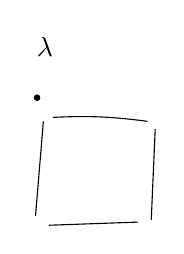
\begin{tikzpicture}[x=1cm,y=1cm]
\node at (0,2.25) {$\lambda$};
\fill (-0.1,1.6) circle (1.2pt);
\draw (0.1,1.35) to[bend left=5] (1.3,1.3);
\draw (-0.02,1.3)--(-0.12,0.1);
\draw (1.4,1.2)--(1.35,0.05);
\draw (0.05,-0.02)--(1.18,0.02);
\end{tikzpicture}}
\[
(\lambda(x)+v(y))^2+Q(y)
\]
\[
\lambda^2x^2+v(y)^2=\unsure{X^2|x^2}
\]
\[
v(y)^2=0
\]
\[
\lambda^2=1
\]
\[
v(y)^2=
\]
\[
\uline{\lambda^2=1}\qquad\mu_2
\]
\diagram{\[
\left(\begin{array}{ccccc}
\mu_2&\alpha_2&\alpha_2&\mathbin{-}\mathbin{-}&\alpha_2\\[1cm]
&&&&
\end{array}\right)
\]}

$\deleted{\unsure{x\longmapsto\lambda}}$
\[
(\xi,\unsure{x|y})\longrightarrow(\lambda\xi+u(y),y)
\]
\[
\lambda^2=1\qquad u(y)^2=0
\]
\[
\lambda'\lambda\xi+\lambda'u(y)+u'(y)
\]
\[
(\lambda',u')(\lambda,u)=(\lambda'\lambda,\lambda'u+u')
\]
\[
\mu_2.
\]
}
\margin{63}
\scanpage{66}
formes bilinéaires sym. forment un anneau
\[
\left\{\begin{array}{l}
\text{les formes \unsure{alternées} un module sur cet anneau}\\
\text{les formes quadratiques également}
\end{array}\right.
\]

\deleted{\unsure{?}} On a un
\diagram{
\begin{tikzcd}[ampersand replacement=\&,column sep=large,row sep=large]
H^1(S,\mu_2)\arrow[dr]\&\&\\
\&\text{Bil}\deleted{\arrow[dd,bend right=60,"\alpha"']}\&\lambda\text{ anneau}\ \deleted{\unsure{pour}}\\
\&\text{Alt}\&\text{Module}\\
\&\text{Quad}\deleted{\arrow[uu,bend left=30,"\beta"]}\&\text{Module}\arrow[uu,bend right=25,"\pi"']
\end{tikzcd}
}
\[
\left.\operatorname{Bil}+\operatorname{Alt}\right|\ \lambda\text{-module gradué par }\mathbb Z/2\mathbb Z
\]
muni d'un élément \uline{privilégié} \unsure{d'aug.|dim.} $2$

muni d'un \unsure{élément} \unsure{privilégié} \unsure{d'aug.|dim.} $1$

\margin{$A\qquad M$
\[
f(x,y)z=xf(\unsure{yz|y,z})
\]
}

\deleted{$\lambda$-anneau}\quad $\lambda^2$
\[
(Q\otimes f')(\sum x_i
\]
\deleted{\unsure{sur}}\quad$\mathbin{-}$
\[
\deleted{Q(x\wedge y)=}
\]
\[
f\unsure{\sim|\rightsquigarrow} Q
\]
\[
f(x\wedge y,x\wedge y)=\begin{pmatrix}f(x,x)&f(x,y)\\f(y,x)&f(y,y)\end{pmatrix}=Q(x,x)Q(y,y)-f(x,y)^2
\]
\[
Q(x\wedge y)=Q(x,x)Q(y,y)-f(x,y)^2
\]
\[
\deleted{\alpha(Q\otimes}
\]
\[
\deleted{\alpha(f\otimes f')=}\qquad\alpha(f)=f\otimes\alpha(1)
\]
\[
\beta(\unsure{'}
\]

\margin{
\figure{\begin{tikzpicture}[x=1cm,y=1cm]
\draw (-0.6,0)--(1.1,0);
\draw (0,-0.55)--(0,1.2);
\draw[line width=1pt] (0,0)--(0,1.1);
\fill (0,1.1) circle (1.4pt);
\node[above right] at (0,1.1) {\deleted{\unsure{ad}}};
\end{tikzpicture}}
\[
\deleted{\unsure{ax^2}}
\]
\[
e_1e_2=e_1^2=0
\]
\[
\deleted{(xe_1+ye_2),(x'e_1+y'e_2)}=yy'
\]
\[
\deleted{(e_1+e_2)(e_1+e_2)}\qquad e_1+e_2\mathbin{-}+e_n
\]
\[
\sum x_i^2=\unsure{0}
\]
\[
\underbrace{e'_1}_{\text{carré }1}\quad\underbrace{e'_2\ e'_3\mathbin{-}e'_n}_{\text{carré nul}}\quad\deleted{\unsure{e_n}}\quad\deleted{\text{carré }1}
\]
\[
\deleted{e_1\mathbin{-}\unsure{e_2}}
\]
\[
e_1,\ e_1-e_2,\ e_1-e_3,\ \mathbin{-},\ e_1-e_n
\]
\[
e'_ie'_j=0\quad\unsure{i,j\ne1}
\]
\[
(e_1-e_i)(e_1-e_j)=1\ \deleted{\unsure{+0}}
\]
\[
a_{11}x_1x'_1+\sum_{\substack{\deleted{\unsure{i\ne j}}\\\deleted{\unsure{i,j\ne1}}\\\inserted{1\leq i<j}}}\unsure{a_{ij}}(x_ix'_j+x_jx'_i)
\]
\[
a_{11}x_1x'_1\ \deleted{\unsure{+}}
\]
}
\margin{65}
\scanpage{67}
- \mspage{108} -
\hfill n°371
\[
\langle z,u\llcorner(s\wedge t)\rangle=\langle(s\wedge t)\wedge z,u\rangle=\langle t\wedge z,u\llcorner s\rangle=\langle z,(u\llcorner s)\llcorner t\rangle
\]
en vertu de l'associativité de la multiplication dans $\bigwedge(M)$ ; d'où
\[
(31)\qquad u\llcorner(s\wedge t)=(u\llcorner s)\llcorner t.
\]
On peut donc dire que l'application $(t,u)\longrightarrow u\llcorner t$ définit (avec l'addition) une structure de $\bigwedge(M)$-\uline{module à droite gradué} sur $\bigwedge(M)^{*\mathrm{gr}}$ (quand on munit $\bigwedge(M)$ de la graduation \uline{opposée} à celle définie au n°1).

Soit maintenant $f:M\longrightarrow N$ une application $A$-linéaire ; pour $z,t$ dans $\bigwedge(M)$ et $u'\in\bigwedge(N)^{*\mathrm{gr}}$, on a par définition
\[
\begin{aligned}
\langle t\wedge z,{}^{\mathrm t}(\bigwedge(f))(u')\rangle&=\langle(\bigwedge(f))(t\wedge z),u'\rangle=\\
&=\langle(\bigwedge(f))(t)\wedge(\bigwedge(f))(z),u'\rangle=\langle(\bigwedge(f))(z),u'\llcorner(\bigwedge(f))(t)\rangle=\\
&=\langle z,{}^{\mathrm t}(\bigwedge(f))(u'\llcorner(\bigwedge(f))(t)\rangle
\end{aligned}
\]
d'où
\[
(32)\qquad{}^{\mathrm t}(\bigwedge(f))(u'\llcorner(\bigwedge(f))(t))={}^{\mathrm t}(\bigwedge(f))(u')\llcorner t.
\]
En particulier, si $f$ est un \uline{isomorphisme} de $M$ sur $N$, on a
\[
(33)\qquad{}^{\mathrm t}(\bigwedge(f))^{-1}(u\llcorner t)=({}^{\mathrm t}(\bigwedge(f))^{-1}(u))\llcorner((\bigwedge(f))(t))
\]
quels que soient $t\in\bigwedge(M)$, $u\in\bigwedge(M)^{*\mathrm{gr}}$ (formule qui résulte aussi du transport de structure par $f$).

* Nous verrons au §6, n°4 que si $u=x_1^*x_2^*\ldots x_q^*$, où les $x_i^*$ appartiennent à $M^*$, on a, pour tout $t\in\bigwedge^pM$ ($p\leq q$)
\[
(34)\qquad(x_1^*x_2^*\ldots x_q^*)\llcorner t=\sum_H\unsure{\rho|\varepsilon}_{H,K}\langle t,x_H^*\rangle x_K^*
\]
où $H$ parcourt l'ensemble des parties à $p$ éléments de $\lbrack\!\lbrack1,q\rbrack\!\rbrack$, $K$ est le complémentaire de $H$ dans $\lbrack\!\lbrack1,q\rbrack\!\rbrack$ et, pour toute partie $J$ de $\lbrack\!\lbrack1,q\rbrack\!\rbrack$, on pose $x_J^*=x_{i_1}^*x_{i_2}^*\ldots x_{i_m}^*$ si $(i_h)_{1\leq h\leq m}$ est la suite strictement croissante des éléments de $J$. *

Montrons maintenant que, pour $u\in\bigwedge(M)^{*\mathrm{gr}}$, il existe un endomorphisme canonique $s\longrightarrow u\lrcorner s$ du $A$-module $\bigwedge(M)$ tel que l'on ait
\margin{66}
\scanpage{68}
\diagram{
\begin{tikzcd}[ampersand replacement=\&,column sep=small,row sep=large]
\unsure{0}\arrow[r,dash]\&\begin{gathered}\frac{\unsure{n(n+1)|n(m+1)}}2\\\Sigma^2(\check E)\end{gathered}\arrow[rr]\arrow[dr,"\text{surj}"']\&\&\begin{gathered}\frac{\unsure{n(n+1)}}2\\\operatorname{Sym}^2(E)\end{gathered}\arrow[rr]\arrow[dr,"\text{surj}"']\&\&\unsure{\Sigma^2|\Sigma_2}(\check E)\arrow[rr]\arrow[dr,"\text{surj}"']\&\&\begin{gathered}\deleted{x\otimes y}\\\operatorname{Sym}^2(E)\end{gathered}\\
\&\&\check E^{(2)}\arrow[ur,"\text{inj}"]\&\&\check E^{(2)}\arrow[ur,"\text{inj}"]\&\&\check E^{(2)}\arrow[ur,"\text{inj}"]\&
\end{tikzcd}
}

\margin{
\[
\mathbb R
\]
\[
\mathbb C=\mathbb R[i]
\]
\[
\mathbb K=\mathbb R[i,j,k]=\mathbb C\mathbin{\overset{\unsure{\tau}}{\otimes}}\mathbb C
\]
\[
\deleted{M_2(\mathbb C)}
\]
\[
\deleted{M_2(\mathbb K)}
\]
}

\[
\sum a_{ij}x_ix_j\rightsquigarrow\sum a_{ij}x_i\otimes x_j
\]

\diagram{
\begin{tikzcd}[ampersand replacement=\&,column sep=small,row sep=large]
0\arrow[r,dash]\&\operatorname{Alt}^2(\check E)\arrow[r]\&\Sigma^2(\check E)\arrow[rr]\arrow[dr]\&\&\operatorname{Sym}^2(\check E)\arrow[r]\&\operatorname{Alt}^2(\check E)\arrow[r]\&0\\
\&\&\&\check E^{(2)}\arrow[ur]\&\&\&
\end{tikzcd}
}
\diagram{
\begin{tikzcd}[ampersand replacement=\&,column sep=small,row sep=large]
0\arrow[r,dash]\&\check E^{(2)}\arrow[r]\&\operatorname{Sym}^2(\check E)\arrow[rr]\arrow[dr]\&\&\Sigma^2(\check E)\arrow[r]\&\check E^{(2)}\arrow[r]\&0\\
\&\&\&\operatorname{Alt}^2(\check E)\arrow[ur]\&\&\&
\end{tikzcd}
}
\diagram{
\[
\boxed{\begin{gathered}\begin{tikzcd}[ampersand replacement=\&,column sep=large]
\operatorname{Im}=\operatorname{Ker}=\operatorname{Alt}^2(\check E)\&\Sigma^2(\check E)\arrow[r,bend left=12]\&\operatorname{Sym}^2(\check E)\arrow[l,bend left=12]\&\operatorname{Im}=\operatorname{Ker}=\unsure{\check F|\check E}^{(2)}
\end{tikzcd}\end{gathered}}
\]
}

\unsure{alter} $+$ Alternée $+$ \unsure{quad} $+$ \unsure{bilin. prod.}

\deleted{\unsure{Ortho}}
\[
\left\{\begin{array}{l}
\text{Formes quadratiques}\\
\text{Formes bilinéaires symm}
\end{array}\right.
\]
\[
\left\{\text{Formes \deleted{symplectiques}\inserted{alternées}}\right.
\]
\[
\sum x_i
\]
\[
f\otimes f'(x\otimes x',y\otimes y')=f(x,y)f'(x',y')
\]

\diagram{\[
\left\{\begin{array}{rcl}
\text{Forme \deleted{symplectique}\inserted{Alternée}}\otimes\text{Forme \deleted{symplectique}\inserted{Alternée}}&\longrightarrow&\text{forme \deleted{symplectiques}\deleted{\inserted{bilinéaire}}\inserted{bilinéaire}}\\
\text{forme alternée}\otimes\text{forme bil.}&\longrightarrow&\text{forme Alternée}\
\\
\text{forme bil}\otimes\text{forme bil}&\longrightarrow&\text{forme bil.}
\end{array}\right.
\]}
\diagram{\[
\begin{array}{rcl}
\text{Forme quadratique}\otimes\text{forme bil.}&\longrightarrow&\text{forme quadr.}\\
\text{forme quadratique}\otimes\text{forme Alternée}&\longrightarrow&\text{forme Alternée}\\
\text{Forme quadratique}\otimes\text{forme quadratique}&\multicolumn{2}{l}{\ ?!\unsure{?}}
\end{array}
\]}
\margin{67}
\scanpage{69}
- \mspage{109} -
\hfill n°371
\[
(35)\qquad\langle u\lrcorner s,v\rangle=\langle s,vu\rangle
\]
quel que soit $v\in\bigwedge(M)^{*\mathrm{gr}}$.

On notera qu'il existe en général plusieurs endomorphismes distincts de $\bigwedge(M)$ ayant cette propriété, puisqu'il peut y avoir des éléments $\ne0$ de $M$ orthogonaux à $M^*$. Toutefois, si $M$ est un $A$-module \uline{libre}, il en est de même de $\bigwedge(M)$ (n°3, prop.8), donc il n'y a aucun élément $\ne0$ de $\bigwedge(M)$ orthogonal à son dual, et l'application $s\longrightarrow u\lrcorner s$ est bien la restriction à $\bigwedge(M)$ (considéré comme sous-module du dual de $\bigwedge(M)^{*\mathrm{gr}}$) de la \uline{transposée} de l'endomorphisme $v\longrightarrow vu$ de $\bigwedge(M)^{*\mathrm{gr}}$.

Nous définirons l'application linéaire $\bigwedge(M)\otimes\bigwedge(M)^{*\mathrm{gr}}\longrightarrow\bigwedge(M)$ correspondant à l'application bilinéaire $(s,u)\longrightarrow u\lrcorner s$ comme la composée
\diagram{
\begin{tikzcd}[ampersand replacement=\&,column sep=large]
\bigwedge(M)\otimes\bigwedge(M)^{*\mathrm{gr}}\arrow[r,"\Delta\otimes1"]\&\bigwedge(M)\otimes\bigwedge(M)\otimes\bigwedge(M)^{*\mathrm{gr}}\arrow[r,"1\otimes p"]\&\bigwedge(M)
\end{tikzcd}
}
où $\Delta$ a été définie au n°4 et $p:\bigwedge(M)\otimes\bigwedge(M)^{*\mathrm{gr}}\longrightarrow A$ correspond à la forme bilinéaire canonique (chap.II, 3e éd., §2, n°\quad). Si $s=x_1\wedge x_2\wedge\ldots\wedge x_p$, $u\in(\bigwedge^qM)$, il résulte déjà de cette définition que $u\lrcorner s=0$ si $q>p$ ; si $q\leq p$, la formule (9) du n°3 appliquée pour $n=2$ et avec tous les $x_{ji}$ ($1\leq i\leq n$) égaux à un même élément $x_j$ ($1\leq j\leq m$) donne, pour la composante de $\Delta(s)$ dans $(\bigwedge^{p-q}M)\otimes(\bigwedge^qM)$, l'élément $\sum_H\unsure{\rho|\varepsilon}_{K,H}x_K\otimes x_H$, où $H$ parcourt l'ensemble des parties à $q$ éléments de $\lbrack\!\lbrack1,p\rbrack\!\rbrack$ et $K$ est le complémentaire de $H$ dans $\lbrack\!\lbrack1,q\rbrack\!\rbrack$ ; d'où
\[
(36)\qquad u\lrcorner s=\sum_H\unsure{\rho|\varepsilon}_{K,H}\langle x_H,u\rangle x_K\ ;
\]
la formule (35) résulte alors aussitôt de (20). On dit que $u\lrcorner s$ est le \uline{produit intérieur gauche} de $u$ et de $s$ ; si $u\in(\bigwedge^qM)^*$, $s\longrightarrow u\lrcorner s$ est une application linéaire \uline{homogène de degré} $-q$. Lorsque $s\in\bigwedge^pM$, $u\in(\bigwedge^pM)^*$, on a $u\lrcorner s=\langle s,u\rangle$.

Pour deux éléments $u,v$ de $\bigwedge(M)^{*\mathrm{gr}}$, on a
\[
(37)\qquad(uv)\lrcorner s=u\lrcorner(v\lrcorner s)
\]
autrement dit, l'application $(u,s)\longrightarrow u\lrcorner s$ définit (avec l'addition) une structure de $\bigwedge(M)^{*\mathrm{gr}}$-\uline{module à gauche gradué} sur $\bigwedge(M)$, quand on munit $\bigwedge(M)^{*\mathrm{gr}}$ de la
\margin{68}
\scanpage{70}
$E^{2n}(S)=$ ens des classes de couples $(E,F)$, $E$ et $F$ formes quadratiques \unsure{admissibles} de \unsure{rangs} \deleted{\unsure{2n}} \inserted{\uuline{pairs}} telles que $\operatorname{rang}E-\operatorname{rang}F=$
\[
x_1^2+\text{---}+x_n^2+\deleted{xy}\;y_1y_2+y_3y_4\text{---}+y_{2m-1}y_{2m}
\]
$\bar E^{n,m}=$ ens des classes à isom près des formes quadratiques \unsure{pointées} de type $(n,m)$
\[
\coprod_{n,m\geq0}\bar E^{n,m}(S),=\bar E(S)
\]
est muni d’une structure de \uline{monoïde} \uline{bigradué}.

\deleted{Soit} [N.B. Si $2$ est \unsure{inv.} alors $\bar E^{\unsure{n},m}\simeq\bar E^{\deleted{\unsure{m}}n+2m,0}$

Si $2=0$, \deleted{$\unsure{A\text{---}0}$}, alors $\bar E^{n,m}\simeq\bar E^{1,m}$ ;

\deleted{\unsure{mais}}

en particulier, \unsure{on ne peut retrouver|on ne peut reconnaître} : \deleted{\unsure{l’isom.}}
\[
\unsure{E\simeq}E^{\alpha,0}\quad\text{ou}\quad E^{1,\beta},\quad\text{ou}\quad E^{0,\unsure{\gamma}}\text{---}\quad]
\]
$E(S)$ groupe associé au monoïde
\[
\deleted{\coprod_{n,m\in\mathbb Z}\bar E^{n,m}(S)}
\]
\diagram{\begin{tikzcd}[ampersand replacement=\&]
E(S)\arrow[r,"\epsilon_1\times\epsilon_2"]\&\mathbb Z\times\mathbb Z
\end{tikzcd}}
\[
E^{n,}
\]
\margin{69}
\scanpage{71}
-\mspage{122}-
\margin{n° 371}
\uline{mineurs d’ordre} $p$ (\uline{pour} $p\leq\inf(m,n)$) \uline{les déterminants des matrices carrées d’ordre} $p$ \uline{obtenues à partir des sous-matrices à} $p$ \uline{lignes et} $p$ \uline{colonnes de la matrice $X$}.

Etant donnée une sous-matrice de $\underline X$ à $p$ lignes et $p$ colonnes, les diverses matrices carrées que l’on en déduit ne différant que par l’ordre des lignes ou des colonnes ; leurs déterminants sont donc les mêmes \uline{au signe près}. \uline{Dans toute la suite de ce chapitre}, nous nous bornerons au cas où $\underline X$ est une matrice dont l’ensemble des indices des lignes est l’intervalle $\lbrack\!\lbrack1,m\rbrack\!\rbrack$ de $N$ et l’ensemble des indices des colonnes l’intervalle $\lbrack\!\lbrack1,n\rbrack\!\rbrack$ de $N$. Soit alors $H$ (resp. $K$) une partie de $p$ éléments de l’ensemble $\lbrack\!\lbrack1,m\rbrack\!\rbrack$ (resp. $\lbrack\!\lbrack1,n\rbrack\!\rbrack$) et considérons la sous-matrice de $\underline X$ obtenue en supprimant dans $\underline X$ les lignes d’indice $i\in\complement H$ et les colonnes d’indice $j\in\complement K$ ; nous désignerons par $X_{H,K}$ le déterminant de la matrice carrée obtenue à partir de la sous-matrice précédente en \uline{rangeant par ordre croissant} les indices de ses lignes et de ses colonnes. Soit $(i_h)_{1\leq i\leq p}$ (resp. $(j_k)_{1\leq k\leq p}$) la suite strictement croissante des éléments de $H$ (resp. $K$) ; la définition précédente équivaut donc à la relation
\[
\begin{split}
(9)\quad &(e_{i_1}\xi_{i_1j_1}+e_{i_2}\xi_{i_2j_1}+\ldots+e_{i_p}\xi_{i_pj_1})\wedge\ldots\wedge(e_{i_1}\xi_{i_1j_p}+e_{i_2}\xi_{i_2j_p}+\ldots+e_{i_p}\xi_{i_pj_p})=\\
&=X_{H,K}.e_{i_1}\wedge e_{i_2}\wedge\ldots\wedge e_{i_p}.
\end{split}
\]
PROPOSITION 5.- \uline{Soit} $M$ \uline{un A-module ayant une base} $(e_i)_{1\leq i\leq n}$ \uline{de} $n$ \uline{éléments, et pour tout} $p\leq n$, \uline{soit} $(e_H)$ \uline{la base correspondante de} $\bigwedge^pM$, $H$ \uline{parcourant l’ensemble des parties de} $\lbrack\!\lbrack1,n\rbrack\!\rbrack$ \uline{à} $p$ \uline{éléments} (§ 5, n°\inserted{\unsure{3}}, prop.8). \uline{Soit} $(x_j)_{1\leq j\leq p}$ \uline{une suite de} $p$ \uline{éléments de} $M$, \uline{et soit $X$ la matrice à} $n$ \uline{lignes et} $p$ \uline{colonnes dont les composantes} $\xi_{ji}$ $(1\leq i\leq n)$ \uline{de} $x_j$ \uline{sur la base} $(e_i)$ \uline{forment la colonne d’indice} $j$. \uline{Alors la composante du} $p$-\uline{vecteur décomposable} $x_1\wedge x_2\wedge\ldots\wedge x_p$ \uline{sur} $e_H$ \uline{est le mineur} $X_{H,J}$ \uline{de $X$, où} $J=\lbrack\!\lbrack1,p\rbrack\!\rbrack$ (que l’on écrit aussi simplement $X_H$).

Cela résulte aussitôt de la formule (9), où on fait $j_k=k$ pour $1\leq k\leq p$ et où
\margin{70}
\scanpage{76}
Formes quadratiques

(Exposé de Kneser à l’IHES)
\margin{\textcircled{1} \uline{Généralités}}

$A$ anneau commutatif

$E(A)$ anneau des formes quadratiques ``non dégénérées'' [i.e. à discriminant non div de $0$] sur modules projectifs de type fini

$F(A)$ anneau des formes quadratiques ``unimodulaires'' [i.e. à discriminant inversible]

Si $A$ est un corps, $E(A)=F(A)$

\uline{Invariants pour} $F(A)$

1°) Rang \quad $\epsilon:F(A)\longrightarrow\mathbb Z$ \quad hom d’anneaux

2°) Discriminant \quad $d:F(A)\longrightarrow A^*/A^{*2}$ \quad hom de groupes

3°) Classe de Clifford \quad $c:F(A)\longrightarrow{}_2\operatorname{Br}(A)$ \quad application

La définition de $c$ par Kneser se fait en le définissant d’abord pour un module quadratique [en distinguant le cas pair, on prend $\operatorname{Cl}(E)$, et impair, on prend $\operatorname{Cl}^{+}(E)$], puis on \unsure{note} que si $E$ et $E'$ ont \deleted{de rang} discriminant unité, alors $c(E+E')=c(E)+c(E')$, donc on peut définir $c$ au moins sur le sous-groupe $\unsure{F^2(A)|\Gamma^2(A)}$ noyau de $\epsilon,d$ ----

[N.B. Lorsque $A$ est local de car rés $\neq2$, on peut donner une définition des $w_i$ de Stiefel-Whitney, redonnant $d$ et $c$ -----
\margin{75}
\scanpage{77}
$\epsilon,d,c$ donnent une filtration de $F(A)$
\[
F(A)/F_1(A)\unsure{=|\simeq}\mathbb Z
\]
\diagram{\(\begin{array}{l}\left.\begin{array}{l}
F_1(A)/F_2(A)\simeq A^*/A^{*2}\\
F_2(A)/F_3(A)\subset{}_2\operatorname{Br}(A)
\end{array}\right\}\quad\begin{array}{l}\text{dans le cas $A$ un corps}\\\text{de car. $\neq2$}\end{array}
\end{array}\)}
\inserted{\diagram{\begin{tikzcd}[ampersand replacement=\&,column sep=small,row sep=0pt]\phantom{F_3(A)}\arrow[r,bend right=18] \& \begin{array}{l}\text{sous-groupe des}\\\text{éléments décomposables}\end{array}\end{tikzcd}}}

\deleted{$\unsure{F_1}$}

A-t-on en tout cas pour corps de car. arbitraire
\[
\left\{\begin{array}{l}
F_1(A)/F_{\unsure{1|2}}(A)\simeq H^1(A,\mathbb Z/2\mathbb Z)\\
F_2(A)/F_3(A)\subset H^2(A,\mathbb Z/2\mathbb Z)
\end{array}\right.
\]
\margin{76}
\scanpage{78}
\margin{\textcircled{2}}
\uline{Exemples \inserted{\figure{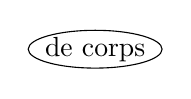
\begin{tikzpicture}[baseline=(n.base)]\node (n) {de corps};\draw (n.center) ellipse (0.85cm and 0.24cm);\end{tikzpicture}}} d’anneaux} (Cas de corps \deleted{\unsure{de}} de car $\neq2$)

\diagram{\(\begin{array}{llll}
\text{a) \uline{corps alg. clos} }k&F(k)\simeq\mathbb Z&[\text{\unsure{i.e.}}\ F_1(k)=0\ ]\\[3pt]
\text{b) \uline{Corps fini} }K&F(k)\simeq\mathbb Z+\mathbb Z/2\mathbb Z&[\text{\unsure{i.e.}}\ F_2^{\deleted{3}}(k)=0\ ]\\[3pt]
\text{\unsure{b|c}) \uline{Corps} }\uline{p\text{-adiques}}\ K&F(K)\simeq\mathbb Z\ \begin{array}{l}\text{étendu par un}\\\text{groupe fini}\\\text{annulé par $4$}\end{array}&[\text{\unsure{i.e.}}\ F_3(k)\unsure{=0}\ ]\\[3pt]
\text{d) \uline{Corps} }\mathbb R&\begin{array}{l}F_1(k)\simeq\mathbb Z\\\text{par l’index}\\F_2(k)=2\mathbb Z\\F_3(k)=4\mathbb Z\end{array}&\deleted{\unsure{F_2}}
\end{array}\)}

e) Corps valué complet à corps résiduel alg clos \deleted{\unsure{discrètement}}
\[
F_{\unsure{k|1}}(K)\simeq\mathbb Z+\underbrace{K^*/k^{*2}}_{\mathbb Z/2\mathbb Z}\qquad[\text{On a }F_2(k)=0]
\]
\margin{si car. résiduelle est $\neq2$, \unsure{quasi par définition...}}

\margin{\textcircled{3}}
\deleted{\unsure{3}} \uline{Corps de nombres}

\uline{Th. de Hasse}
\diagram{\begin{tikzcd}[ampersand replacement=\&,column sep=large]
F(K)\arrow[r]\&\sum_pF(K_p)\&\text{\uuline{injectif}}\\
F_1(K)/F_2(K)\arrow[r]\&\sum_pK_p^*/K_p^{*2}\&\begin{array}{l}\text{injectif [grâce à Hasse}\\\text{\unsure{égalemt}] }\end{array}\\
\underline{F_2(K)/F_3(K)}\arrow[r]\&\sum_p\mathbb Z/2\mathbb Z\&\begin{array}{l}\text{injectif [car }\operatorname{Br}(K)\\\subset\sum_p\operatorname{Br}(K_p)]\end{array}
\end{tikzcd}}
\inserted{\diagram{\begin{tikzcd}[ampersand replacement=\&,column sep=small,row sep=small]\&\phantom{F_2(K)/F_3(K)}\\\begin{array}{l}\text{sous-groupe des}\\\text{\unsure{formes d’invariant de norme}}\\\text{unité}\end{array}\arrow[ur,bend right=24]\end{tikzcd}}}
\[
F_3(K)\subset\sum_{\substack{p\text{ infini}\\\text{réel}}}F_3(K_p)\subset\mathbb Z^r
\]
\margin{$r$ nb de places réelles}

Le sous-groupe de torsion de $F(K)$ est le noyau de
\diagram{\begin{tikzcd}[ampersand replacement=\&]
F_1(K)\arrow[r,"\text{index}","\substack{\text{aux places}\\\text{réelles}}"']\&\mathbb Z^r
\end{tikzcd}}
, il est annulé par $4$
\margin{77}
\scanpage{79}
\diagram{\begin{tikzcd}[ampersand replacement=\&]
0\arrow[r]\&E'(A)\arrow[r]\arrow[d,"\unsure{2|?}"]\&E(A)\arrow[r]\arrow[d,no head]\&E(K)\arrow[r]\arrow[d,no head]\&0\\
0\arrow[r]\&\sum\unsure{E^d|E'}(\hat A_p)\arrow[r]\&\sum E(\hat A_p)\arrow[r]\&\sum E(K_p)\arrow[r,no head]\&0
\end{tikzcd}}

\diagram{\begin{tikzcd}[ampersand replacement=\&,column sep=large]
\&\begin{array}{l}\operatorname{Pic}(A)/2\operatorname{Pic}(A)\subset H^2(A,\mu_2)\end{array}\arrow[d,phantom,"\unsure{\Vert|\wr}" description]\&\&E(K)\arrow[d,equal]\\
0\arrow[r]\&F'(A)\arrow[r]\&F(A)\arrow[r,no head]\arrow[d]\&F(K)\arrow[d]\&\deleted{\unsure{\text{---}}}\\
\&0\arrow[r]\&\sum F(\hat A_p)\arrow[r,"\text{inj}"']\&\sum F(K_p)
\end{tikzcd}}
\margin{A anneau de Dedekind ----}

\deleted{\figure{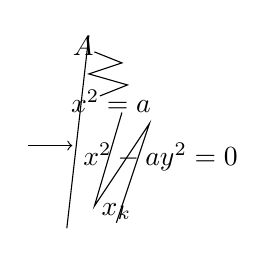
\begin{tikzpicture}[x=.7cm,y=.7cm]
\node at (0,3){$A$};\node at (.5,2){$x^2=\unsure{a}$};
\node at (1.4,1){$\unsure{x^2}-ay^2=0$};\node at (.6,0){$\unsure{x_k}$};
\draw[->](-1,1.2)--(-.2,1.2);\draw(.1,3.2)--(-.3,-.3);
\draw(.2,2.9)--(.7,2.7)--(.1,2.5)--(.8,2.3)--(.3,2.1);
\draw(.7,1.8)--(.2,.1)--(1.2,1.6)--(.6,-.2);
\end{tikzpicture}}}

\margin{$\unsure{\mathbb Q|\mathbb Z}/2\mathbb Z$}
\deleted{\diagram{\begin{tikzcd}[ampersand replacement=\&]
H^1(A,\mathbb Z/2\mathbb Z)\arrow[r]\&\sum_pH^1(\hat A_p,\mathbb Z/2\mathbb Z)\\
H^1(K,\unsure{G_m|\mathbf G_m})\arrow[r]\&{}
\end{tikzcd}}}
\deleted{\diagram{\begin{tikzcd}[ampersand replacement=\&]
0\arrow[r]\&T\arrow[r]\&JT\arrow[r]\&\unsure{MT|M_T}\arrow[r,no head]\&0\\
\unsure{K} \&0\arrow[r,no head]\&L^*\arrow[r]\&J_L\arrow[r,no head]\&C_L\arrow[r,no head]\&0\\
\&0\arrow[r,no head]\&L^*\otimes X\arrow[r,no head]\&J_L\otimes X\arrow[r,no head]\&C_L\otimes X\arrow[r]\&0
\end{tikzcd}}}
\deleted{\[
\unsure{H^1}\qquad H^{\unsure{1}}(G,\ \longrightarrow\ H^{\unsure{1}}(
\]}
\deleted{\[
\sum_pH^1(G_p,\unsure{L_p^*|K_p^*}\otimes X)\longrightarrow
\]}
\deleted{\[
H^{\unsure{1}}(G,K^*)\longrightarrow H^{\unsure{1}}(G,J)
\]}

$\unsure{E'|E^d}(V)$ \inserted{\diagram{\begin{tikzcd}[ampersand replacement=\&,column sep=small,row sep=small]\&\begin{array}{l}\text{anneau de val. discrète}\\\text{complet}\end{array}\\\phantom{V}\arrow[ur,bend left=22]\end{tikzcd}}} est isomorphe à la somme directe d’une infinité de copies de $\unsure{F(k)|E(k)}$, avec $k$ le corps résiduel
\margin{78}
